\documentclass[11pt]{article}
\usepackage{amssymb}
\usepackage{latexsym}
\usepackage{amsmath}
\usepackage{amsthm}
\usepackage{mathtools}
\usepackage{natbib}
\usepackage{tikz-cd}
\usepackage{enumitem} 
\usepackage{hyperref}
\hypersetup{
    colorlinks,
    citecolor=black,
    filecolor=black,
    linkcolor=black,
    urlcolor=black
}
\newtheorem{thm}{Theorem}[section]
\newtheorem{prop}[thm]{Proposition}
\newtheorem{lemma}[thm]{Lemma}
\newtheorem{cor}[thm]{Corollary}
\newtheorem{dfn}[thm]{Definition}
\newtheorem{axiom}[thm]{Axiom}

\newtheorem{rmk}[thm]{Remark}
\newtheorem{ex}[thm]{Example}
\newtheorem{question}[thm]{Question}
\newtheorem{problem}[thm]{Problem}
\renewcommand{\baselinestretch}{1.05}
\newcommand{\reals}{\mathbb R}
\newcommand{\cplx}{\mathbb C}
\newcommand{\intg}{\mathbb Z}
\newcommand{\ratl}{\mathbb Q}
\newcommand{\torus}{\mathbb T}
\newcommand{\frakg}{{\mathfrak g}}
\newcommand{\frakd}{{\mathfrak d}}
\newcommand{\calf}{{\cal F}}
\newcommand{\calg}{{\cal G}}
\newcommand{\cala}{{\cal A}}
\newcommand{\calc}{{\cal C}}
\newcommand{\cale}{{\cal E}}
\newcommand{\call}{{\cal L}}
\newcommand{\calo}{{\cal O}}
\newcommand{\mathbold}{\bf}
\newcommand{\cinf}{C^{\infty}}
\newcommand{\row}[2]{#1_1,\dots ,#1_{#2}}
\newcommand{\dbyd}[2]{{\partial #1\over\partial #2}}
\newcommand{\Space}{{\bf Space}}
\newcommand{\alg}{{\mathbold Alg}}
\newcommand{\pois}{{\mathbold Pois}}
\newcommand{\pitilde}{\tilde{\pi}}
\renewcommand{\qedsymbol}{$\square$}
\bibliographystyle{plain}
\title{\bf Witten Genus on String Toric Complete Intersections}
\author{Lin-Da Xiao %\thanks{Research partially supported by NSF Grant DMS-96-25122 and the Miller Institute for Basic Research in Science.}
{\small(xiaol@student.ethz.ch)}}
\begin{document}
\begin{titlepage}

\includegraphics[width=0.4\textwidth]{Logo}
    \begin{center}
        \vspace*{1cm}
        \begin{Huge}
        \textbf{Witten Genus on String Toric Complete Intersections}
        \end{Huge}
        
        \vspace{1.5cm}
        
        \textbf{Linda Xiao}\\
        \vspace{1cm}
        \text{Advisor: Professor Giovanni Felder}\\
        \text{Co-advisor : Qingtao Chen}
        \vfill
        
        A thesis presented for the degree of\\
        Master of Physics
        
        \vspace{0.8cm}
        
        
        
        Department Physics\\
        Swiss Federal Institute of Technology in Zurich\\
        August 2017
    \end{center}
\end{titlepage}
\newpage
\section*{Acknowledgement}
I am grateful to Doctor Qingtao Chen for a lot of discussion and help on the Witten genus. I also thanks Doctor Honglu Fan for inspiring suggestions.  I would like to thank Professor Ana da Silva for her kind help in clarifying some doubts about symplectic toric variety. Special thank goes to Professor Giovanni Felder. Thanks to his patient discussion and sharp questions, I managed to correct the false understandings of some black-boxes.
\newpage
\maketitle
\tableofcontents
\section{Introduction}
Let $M$ be a $4k$ dimensional closed oriented smooth manifold. In \cite{witten1988index}, Witten genus is defined by formally applying the equivariant Atiyah-Singer Index Theorem to a hypothetical Dirac operator in the loop space and we can get the analogue of $\hat{A}$-genus
\begin{equation*}
	W(M)=\left\langle\hat{A}(TM) Ch(\Theta(T_\mathbb{C}M)),[M] \right\rangle,
\end{equation*}
where 
\begin{equation*}
	\Theta(T_{\mathbb{C}}M)=\underset{m=1}{\overset{\infty}{\bigotimes}} S_{q^{m}}(T_{\mathbb{C}}M-\mathbb{C}^{4k})
\end{equation*}
is the Witten bundle defined in \cite{witten1988index} where $q=e^{2\pi\sqrt{-1} \tau}$ with $Im(\tau)\geq 0$. Also, 
		\begin{equation*}
			S_{q^m} (T_{\mathbb{C}}M-\mathbb{C}^{4k}) :=\sum^\infty_{k=0}(S^k (T_{\mathbb{C}}M-\mathbb{C}^{4k}))(q^m)^k,
		\end{equation*} 
where $S^k(T_\cplx M-\cplx^{4k})$is the k-th symmetric power of the formal difference $T_\cplx M-\cplx^{4k}$ in the K-theory.
To manifest the modular aspects of Witten genus, following \cite{liu1996elliptic}, we can also write it as
\begin{equation*}
	W(M)=\left\langle\prod_{i}\frac{z_i \theta'(0,\tau)}{\theta(z_i,\tau)},[M]\right\rangle
\end{equation*}
where $\{\pm 2\pi\sqrt{-1}z_i,1\leq i\geq 2k\}$ are the formal Chern roots of the bundle $T_{\mathbb{C}}M$.

The oriented manifold $M$ is called \textbf{spin} if the  second Stiefel-Whitney class $w_2(TM)$ vanishes. Moreover, manifold $M$ is called \textbf{string} if the half of the first Pontryagin class vanishes. According to the Atiyah-Singer index theorem, when manifold is spin, the Witten genus is an integral expansion in terms of $q$ (cf. \cite{hirzebruch1992manifolds}). It is also well known that if the manifold is string, the Witten genus is a modular form of weight $2k$ over $SL(2,\mathbb{Z})$ with integral Fourier expansion (\cite{zagier1988note}).
Analogous to Lichnerowicz's classical result on $\hat{A}$ genus (cf. \cite{lawson2016spin}), which stated that $\hat{A}$ genus on spin manifold with positive scalar curvature vanishes, Stolz conjectured that the Witten genus on string manifold with positive Ricci curvature vanishes(for the original arguments, cf. \cite{stolz1996conjecture}, and for a review cf. \cite{dessai2009some}). 

Toward the Stolz's conjecture, several vanishing results have been discovered. There are basically two types of methods. One is to apply the theorem of Dessai \cite{dessai1994witten} which is based on Liu \cite{liu1995modular} when the manifold admits some nontrivial action of a semi-simple Lie group. The current results via this method include:
\begin{enumerate}
\item String homogeneous spaces of compact semi-simple Lie groups \cite{dessai1994witten,liu1995modular}。
\item Total spaces of fiber bundles with fiber $G/H$, with compact semi-simple structure group $G$ \cite{stolz1996conjecture}.
\item Generalized string complete intersection in irreducible, compact, Hermitian, symmetric spaces\cite{forster2007stolz}.
\item String manifold with effective torus action such that $dim\  T>b_2(M)$ \cite{wiemeler2017note}, where $T$ is a compact torus and $b_2(M)$ is the second Betti number of $M$.
\end{enumerate}

Alternatively, sometimes, one can reduce the calculation of Witten genus to calculation of residues. This method was first used by Landweber and Stone \cite{hirzebruch1992manifolds}, which is purely computational and more direct. The vanishing results include:
\begin{enumerate}
\item String complete intersection in projective space\cite{hirzebruch1992manifolds}.
\item String complete intersection in products of projective spaces \cite{chen2008witten}。
\item String complete intersection in products of Grassmannians and flag manifolds\cite{zhou2014witten,zhuang2016vanishing}。
\end{enumerate}
This method also has many applications in elliptic genus\cite{ma2005elliptic,gorbounov2008mirror}.
In this paper we generalize the result of Chen-Han \cite{chen2008witten} to string complete intersections in Toric varieties. We mainly follow the second method in our calculation and also borrow the techniques of equivariant localization in \cite{dessai2016torus}.

\subsection*{Main Result}
Consider a symplectic toric variety $X$ with a set of  invariant divisors $\{D_{\rho_j}\}_{1\leq j\leq r}$ and of Picard number $k$ (For definition of invariant divisors see Definition~\ref{ideals} ). Choose a basis $\{q_1,...,q_k\}$ of the Picard group to expand all the invariant divisors with integer coefficients
\begin{equation*}
D_{\rho_j}=\left\{
\begin{aligned}
& q_j & 1\leq i\leq k\\
& \sum_{i=1}^k m_{j i} q_i  &k+1\leq j\leq r.
\end{aligned}
\right.
\end{equation*}
Consider a smooth complete intersection $Y\subset X$ as a generic intersection of $s$ hypersurfaces $\{Y_l\}_{1\leq l\leq s}$. Each $Y_l$ is dual to the cohomology class $\sum_{j}^k d_{l i} q_i$.
\begin{thm}
When the integer matrix elements $(m_{ji})$ and $(d_{ji})$ satisfy
$$
\sum_{j=1}^n d_{ji} d_{j l}-\sum_{j=k+1}^r m_{ji}m_{j l}=0 \text{  for } i\neq l.
$$
and
$$
\sum_{j=1}^n d_{ji}^2-\sum_{j=k+1}^r m_{ji}^2-1=0,
$$
then the complete intersection $Y$ is string and its Witten genus vanishes.
\end{thm}
The paper is organized as follows: In Section 2, we recall the basic notion of multiplicative genera. In Section 3, we generally discuss the cohomology and characteristic classes on toric varieties. In Section 4 we recall the equivariant localization of toric varieties and use it to prove our main theorem.
\section{Elliptic Genus and Witten Genus}

\subsection{Characteristic Classes}
Following \cite{hirzebruch1992manifolds}, we define the characteristic classes in an axiomatic way. 
\begin{dfn}
	$Vect^\bullet(M)$ is the set of isomorphism classes of vector bundles over manifold $X$. A \textbf{characteristic class} is a map $x$ which associates to each vector bundle $E\rightarrow M$ a cohomology class in $H^\bullet(M, R)$, where $R$ is the coefficient ring (usually $\intg$, $\intg_2$ or $\ratl$). In addition, it also has to satisfy the \text{naturality property}: for any morphism $f:M'\rightarrow M$ and any vector bundle $E\rightarrow M$,
	\begin{equation*}
		x(f^*(E))=f^*(x(E)).
	\end{equation*}
\end{dfn}
	Note that the naturality property indicates that the value of characteristic classes $x(T)\in H^i(M,R),\ i>0$ of a trivial bundle $T=M\times \mathbb{K}^n$ is zero. Considering projection $p: M\rightarrow \{pt\}$, we have $x(T)=x(p^*({pt}\times \mathbb{K}^n))=p^*(x({pt}\times \mathbb{K}^n))=0$.

	In this section we briefly recall the three principal types of characteristic classes, namely, the Stiefel-Whitney classes, Chern classes and the Pontryagin classes. Detailed construction and proofs can be founded in \cite{bott2013differential,milnor1974characteristic}.

	The Stiefel-Whitney class is defined on real vector bundles and takes value in $\intg_2$-cohomology ring. 
	\begin{thm}
	There exists a unique sequence of characteristic classes $\{\omega_i\}_{\geq1}$, which assigns to each real vector bundle $E\rightarrow M$ of dimension $n$ a cohomology class
	 $\omega_i(E)\in H^i(M,\intg_2)$ such that
	\begin{enumerate}[label=(\alph*)]
	\item $\omega_i(E)=0$ if $i>n$,
	\item $\omega(E_1\oplus E_2)=\omega(E_1)\smile\omega(E_2)$, where $\omega:=1+\omega_1+\omega_2+...$,
	\item $\omega_1(\mathcal{L})=1$ in $H^1(\reals P^1,\intg_2)$, where $\mathcal{L}$ denotes the canonical line bundle over $\reals P^1$. 
	\end{enumerate}
	\end{thm}
	The $\omega_i(E)$ is called the $i$-th \textbf{Stiefel-Whitney class} of $E$. And $\omega(E)=1+\omega_1(E)+\omega_2(E)+...\in H^\bullet(M,\intg_2)$ is the \textbf{total Steifel-Whitney class} of $E$. Stiefel-Whitney classes gives the topological obstruction to orientation and spin structure.
	\begin{prop}
		$M$ is a smooth manifold. It is orientable if and only if $\omega_1(TM)$ vanishes.
	\end{prop}

	\begin{prop}
		Let $M$ be an orientable smooth manifold. There exists a spin structure on $M$ if and only if the second Stiefel-Whitney class $\omega_2(TM)$ vanishes.
	\end{prop}

	The axiomatic definition of Chern classes is quite similar, but Chern classes are defined for complex vector bundles and take value in $H^\bullet(M,\intg)$.
	\begin{thm}
	There exists a unique sequence of characteristic classes $\{c_i\}_{\geq1}$, which assigns to each complex vector bundle $E\rightarrow M$ of complex dimension $n$ a cohomology class
	 $c_i(E)\in H^{2i}(M,\intg)$ such that
	\begin{enumerate}[label=(\alph*)]
	\item $c_i(E)=0$ if $i>n$,
	\item $c(E_1\oplus E_2)=c(E_1)\smile c(E_2)$, where $c:=1+c_1+c_2+...$,
	\item $c_1(\mathcal{L}_\cplx)=1$ in $H^1( \mathbb{P}^1,\intg)$, where $\mathcal{L}_\cplx$ denotes the canonical line bundle over $\mathbb{P}^1$. 
	\end{enumerate}
	\end{thm}
	\begin{lemma}
	(Splitting Principle). For and complex vector bundle $E\rightarrow M$, there exist a continuous map $p: Y\rightarrow M$ such that
	\begin{enumerate}[label=(\alph*)]
	\item the induced morphism $p^*:H^\bullet(M,\intg)\rightarrow H^\bullet(Y,\intg)$ is injective, and
	\item the pullback bundle $p^*E\rightarrow Y$ splits into a direct sum of line bundles
		\begin{equation*}
			p^*E=L_1\oplus\cdot\cdot\cdot\oplus L_n,\ n=rank(E).
		\end{equation*}
	\end{enumerate}
	\end{lemma}
	\begin{proof}
	See e.g. Section 3.1 of \cite{hatcher2003vector}.
	\end{proof}
	Because $p^*$ is injective, we can characterize $c(E)$ by $p^*(c(E))$.
	\begin{equation*}
	\begin{aligned}
		p^*(c(E)) & =c(p^*(E))=c(L_1\oplus\cdot\cdot\cdot\oplus L_n)\\
				  & =c(L_1)\cdot\cdot\cdot c(L_n)\\
				  & =(1+c_1(L_1))\cdot\cdot\cdot(1+c_1(L_N))\\
				  & =(1+x_1)\cdot\cdot\cdot(1+x_n),
	\end{aligned}
	\end{equation*}
	where $\{x_i:=c_1(L_i)\}_{i=1,...,n}$ are called the \textbf{formal Chern roots} of $E$. We often formally write
	\begin{equation*}
		c(E)=\prod_i(1+x_i).
	\end{equation*}
	\begin{cor}
		For  any complex vector bundle $E\rightarrow M$ of rank $n$ and any complex line bundle $L\rightarrow M$ with $y=c_1(L)$ we have
		\begin{equation*}
		\begin{aligned}
			c_r(L\otimes E) &=\sum^n_{k=0}(c_k(E))y^{n-k},\\
			c_r(\overline{E}) &=c_r(E^*)=(-1)^k c_k(E),
		\end{aligned}
		\end{equation*}
		where $\overline{E}$ is the conjugate complex vector bundle and $E^*$ is the dual bundle of $E$.
		\end{cor}
		\begin{dfn}
			The \textbf{Chern Character} of rank $n$ complex vector bundle is defined by
			\begin{equation*}
				Ch(E):=\sum^n_i e^{x_i}=\sum^\infty_{k=0}\frac{x_1^k+...+x_n^k}{k!}.
			\end{equation*}
		\end{dfn}
		The Chern character has many nice properties:
		\begin{prop}
			For two complex vector bundle $E$ and $E'$ on $M$,
			\begin{equation*}
			\begin{aligned}
				Ch(E\oplus E')&=Ch(E)+Ch(E'),\\
				Ch(E\otimes E')&+Ch(E)Ch(E').
			\end{aligned}
			\end{equation*}
		\end{prop}
		\begin{proof}
		Directly verify these equations at the level of Chern roots.
		\end{proof}
		Remember that the characteristic is an invariant for isomorphism classes of vector bundle, the above proposition in fact says that the Chern character gives a ring homomorphism between the K-theory and the cohomology ring.
		We define the formal power series
		\begin{equation*}
		\begin{aligned}
			\Lambda_t E&:=\sum^\infty_{k=0}(\Lambda^k E) t^k,\\
			S_t E&:=\sum^\infty_{k=0}(S^k E)t^k.
		\end{aligned}
		\end{equation*} 
		\begin{prop}
			For a complex vector bundle $E\rightarrow M$ of rank $n$ with Chern roots $x_1,...,x_n$, we the the following identities.
			\begin{equation*}
			\begin{aligned}
				Ch(\Lambda_t E)&=\prod^n_{i=1}(1+t e^{x_i}),\\
				Ch(S_t E)&=\prod^n_{i=1}\frac{1}{1-t e^{x_i}}.
			\end{aligned}
			\end{equation*}
		\end{prop}
		\begin{dfn}
			For every real vector bundle $E\rightarrow M$ and for every $k\geq1$, we define \textbf{Pontryagin class} of $E$ the cohomology class
			\begin{equation*}
				p_k(E):=(-1)c_{2k}(E_\cplx)\in H^{2k}(X,\intg).
			\end{equation*}
			The \textbf{total Pontryagin class} is then given by
			\begin{equation*}
				p(E)=1+p_1(E)+...+p_{[n/2]}\in H^\bullet(X,\intg).
			\end{equation*}
		\end{dfn}
		\begin{prop}
			For an $n$-dimensional complex vector bundle $E\rightarrow X$, denote by $E_\reals$ its underlying real vector vector bundle of dimension $2n$. Then
			\begin{equation*}
				E_\reals\otimes_{\reals} \cplx\cong E\oplus\overline{E},
			\end{equation*}
			and thus
			\begin{equation*}
			\begin{aligned}
				c(E_\reals\otimes\cplx)&=c(E\oplus\overline{E}))\\
				&=(1+x_1)...(1+x_n)(1-x_1)...(1-x_n)\\
				&=\prod_i^n(1-x_i^2),\\
			p(E_{\reals} ) & =\prod_i^n(1+x_i^2),\\
			\omega_{2k}(E_\reals) & \equiv c_k(E) \mod 2,\\
			\omega_{odd}& =0.
			\end{aligned}
			\end{equation*}
		\end{prop}
		\begin{proof}
			All the above identities can be proved by first verifying them on line bundle then pass to general case via splitting principle.
		\end{proof}
\subsection{Multiplicative Genera}
\begin{dfn}
	Let $M$ and $M'$ be closed oriented $n$-manifolds. $M$ and $M'$ is said to by \textbf{cobordant} if there exists a compact, oriented $(n+1)$-manifold with boundary $Z$ such that $\partial Z$ is diffeomorphic to $X\sqcup (-M')$, where $(-M')$ has the opposite orientation to $M'$. We write $M\sim_+ M'$. 
\end{dfn}
 The ``cobordant'' is an equivalence relation on the set of closed oriented $n$-manifold. Let $\Omega^{+}_n$ denote the set of equivalence classes. Then $\Omega^+_n$ is endowed with an abelian group structure, with
 \begin{itemize}
 	\item the addition induced by the disjoint union
 	\begin{equation*}
 		[M]+[M']=[M\sqcup M'],
 	\end{equation*}
 	\item the identity $[\emptyset]$ being the cobordant classes of all $n$-dimensional boundaries,
 	\item the inverse of any class $[M]$ given by $[-M]$.
 \end{itemize}
 Moreover, the Cartesian product of two manifolds induces a well-defined operation
 \begin{equation*}
 \begin{aligned}
 	\Omega^+_n\times \Omega^+_m & \longrightarrow \Omega^+_{n+m}\\
 	([N],[M]) & \longmapsto[N\times M].
 \end{aligned}
 \end{equation*}
 The multiplication is obviously distributive over the disjoint union, which renders a graded ring 
 \begin{equation*}
 	\Omega^+_\bullet:=\bigoplus^\infty_{k=0}\Omega_k^+,
 \end{equation*}
 called the \textbf{oriented cobordism ring}.

 \begin{thm}
 	(Thom). The oriented cobordism group $\Omega^+_n$ is finite for $n\not\equiv 0 (\text{mod } 4)$, and is finitely generated group with rank equal to the number of partitions $P(k)$, when $n=4k$.
 \end{thm}
 \begin{proof}
 See Theorem 18.8 of \cite{milnor1974characteristic}.
 \end{proof}
 Then we tensor it with $\mathbb{Q}$ to kill the torsion parts and we get a $\mathbb{Q}$-algebra
 \begin{equation*}
 	\Omega_\bullet^+\otimes \mathbb{Q}=\bigoplus_{k\geq0}^\infty \Omega^+_{4k}\otimes \mathbb{Q},
 \end{equation*}
 which is named \textbf{rational oriented cobordism}.
 \begin{thm}
 	The $\ratl$-algebra is generated by the equivalence classes of 
 	\begin{equation*}
 		\mathbb{P}^{2i_1}\times...\times\mathbb{P}^{2i_r},
 	\end{equation*}
 	with positive integers $i_1,...,i_r$ giving a partition of $k$.
 \end{thm}
 \begin{proof}
 See Corollary 17.5 and related sections in \cite{milnor1974characteristic}.
 \end{proof}
 \begin{dfn}\label{genus}
 	A \textbf{multiplicative genus} is a $\mathbb{Q}$-algebra homomorphism form the rational oriented cobordism to a commutative graded $\mathbb{Q}$-algebra $A$
 	\begin{equation*}
 		\varphi:\Omega^+_\bullet\otimes \mathbb{Q}\longrightarrow A.
 	\end{equation*}
 	i.e. $\varphi$ satisfies:
 	\begin{enumerate}[label=(\alph*)]
 	\item $\varphi(M\sqcup M')=\varphi(M)+\varphi(M')$,
 	\item $\varphi(M\times M')=\varphi(M)\varphi(M')$,
 	\item $\varphi(M)=0$ if $M$ is diffeomorphic to the boundary of compact oriented manifold.
 	\end{enumerate}
 \end{dfn}
 A famous example is the signature of $4k$-manifold M.
 \begin{ex}
 	 For every $4k$-dimensional compact oriented manifold, there is a quadratic form $q_M$ given by
 	 \begin{equation*}
 	 	\begin{aligned}
 	 		H^{2k}(M,\ratl)\times H^{2k}(M,\ratl)& \longrightarrow \ratl\\
 	 		(\alpha,\beta)&\longmapsto (\alpha\smile\beta)[M].
 	 	\end{aligned}
 	 \end{equation*}
 	 and 
 	 \begin{equation*}
 	 	Sig(M):=Sig(q_M).
 	 \end{equation*}
 	 One can verify that $Sig(M)$ satisfies the property (a) in Definition~\ref{genus} because 
 	 \begin{equation*}
 	 	H^\bullet(M\sqcup N,\ratl)\cong H^\bullet(M,\ratl)\oplus H^\bullet(N,\ratl)
 	 \end{equation*}
 	 and it satisfies the property (b) because of the Kunneth formula
 	 \begin{equation*}
 	 	H^{2k}(M\times N,\ratl)\cong\bigoplus^{2k}_{i=0}H^i(M,\ratl)\otimes H^{2k-i}(N,\ratl).
 	 \end{equation*}
 	 For property $(c)$, please refer to \cite{hirzebruch1966topological}.
 \end{ex}

 \begin{dfn}
 	A \textbf{multiplicative sequence} is a sequence of polynomials $\{K_n\}_{n\geq1}$ such that, for every commutative graded unital $\ratl$-algebra $A=\oplus_{k\geq0}A_k$ and every pair of element of the form
 	\begin{equation*}
 		\begin{aligned}
 			a&=1+a_1+a_2+...,\ \ a_i\in A_i,\\
 			b&=1+b_1+b_2+...,\ \ b_i\in A_i,\\
 			&K(ab)=K(a)K(b).
 		\end{aligned}
 	\end{equation*}
 	Here, $K(a)$ is defined by $1+K_1(a_1)+K_2(a_1,a_2)+K_3(a_1,a_2,a_3)+...\in A$.
 \end{dfn}

 \begin{thm}
 	For every formal even power series $Q(x)$, there exists a unique multiplicative sequence $\{K_n\}_{n\geq1}$ such that
 	\begin{equation*}
 		Q(x)=K(1+x^2),
 	\end{equation*}
 	and in turn, every multiplicative genus is determined by the even power series by
 	\begin{equation*}
 	\begin{aligned}
 		Q(x_1)...Q(x_n)& =K(1+x_1^2)...K(1+x_n^2)\\
 			&=K\left(\prod_i^n(1+x_i^2)\right)\\
 			&=K\left(1+p_1+p_2+...p_n\right),
 	\end{aligned}
 	\end{equation*}
 	where $p_i$ is the $i$-th elementary symmetric function of $\{x_j^2\}$.
 \end{thm}
 Recall that for a $4k$-dimensional oriented manifold, the total Pontryagin class can be formally written as
 \begin{equation*}
 p(TM)=(1+x_1^2)\cdot\cdot\cdot(1+x_n^2).
 \end{equation*}
 If we let $\pm x_1,...,\pm x_k$ be the Chern roots of $T_\cplx M$, the elementary symmetric function $p_i$ would just yield the $i$-th Pontryagin class. 
 \begin{dfn} 
 	Let $M$ be an oriented manifold, and $K$ be a multiplicative sequence, we define the \textbf{K-genus} as 
 	\begin{equation*}
 	K[M]:=\left\{
 		\begin{aligned}
 			& K_k(p_1,...,p_k)[M]\in \ratl & \text{if dim }M=4k\\
 			& 0 & \text{if dim } M\not\equiv 0 \mod 4.
 		\end{aligned}
 		\right.
 	\end{equation*}
 	In other word, 
 	\begin{equation*}
 		K[M]=\left\langle\prod^{2k}_1Q(x_i),[M]\right\rangle,
 	\end{equation*}
 	 where $Q(x)$ is the even power series corresponding to $K$ and $x_1,...,x_{2k}$ are the formal Chern roots of $T_\cplx M$.
 	\end{dfn}

 	\begin{thm}
 		The $K$-genus defined above is indeed a multiplicative genus taking value in $\ratl$.
 	\end{thm}
 	\begin{proof}
 		Let $M$ and $N$ be two oriented manifolds of same dimension. The cohomology ring of their disjoint union  gives a direct sum of their cohomology rings. We have
 		\begin{equation*}
 			H^\bullet(M\sqcup N,\intg)\cong H^\bullet(M,\intg)\oplus H^\bullet(N,\intg),
 		\end{equation*}
 		and 
 		\begin{equation*}
 			p_i(T(M\sqcup N)=(p_i(TM),p_i(TN)),
 		\end{equation*}
 		which altogether give the additivity of $K$-genus.

 		Now consider $M$ and $N$ begin two oriented manifold of dimension $m$ and $n$ respectively. On $M\times N$, we have
 		\begin{equation*}
 		T(M\times N)\cong \pi_M^*(TM)\oplus \pi_N^*(TN),
 		\end{equation*}
 		where $\pi_N,\pi_N$ are the natural projections. Using the shorthand notion $p(M):=p(TM)$, the total Pontryagin class of $M\times N$ is 
 		\begin{equation*}
 			p(M\times N)=p(\pi_M^*(TM)\oplus\pi_N^*(TN))=\pi_M^*(p(M))\smile \pi_N^*(p(N)).
 		\end{equation*}
 		$K$ is a multiplicative sequence, which renders
 		\begin{equation*}
 			K(p(M\times N))=K(\pi_M^*(p(M)))\smile K(\pi_N^*(p(N))).
 		\end{equation*}
 		The $K$-genus of the product is then
 		\begin{equation*}
 			\begin{aligned}
 				K[M\times N] & = K_{(m+n)/4}(p_1,...,p_{(m+n)/4})[M\times N]\\
 							&= \sum_{i+j=(m+n)/4}K_i(p_1(M),...,p_i(M))[M]\cdot K_j(p_1(N),...,p_j(N))[N].
 			\end{aligned}
 		\end{equation*}
 		The last term is nonzero only when $i=m/4$ and $j=n/4$, which gives
 		\begin{equation*}
 			K[M\times N]=K[M]K[N].
 		\end{equation*}
 		If either one of $m,n$ is not divisible by 4, $K[M\times N]=K[M]K[N]=0$. So the multiplicativity has been verified.

 		Let $M$ be a $4k$-manifold such that $M$ is the boundary of an oriented $(4k+1)$-manifold with boundary $X$.
 		We denote $[X]$  the fundamental class in $H_{4k+1}(X,\partial X=M,\intg)$, then
 		\begin{equation*}
 			\partial_*([X])=[\partial X]=[M].
 		\end{equation*}
 		Consider the inclusion $\iota: M\hookrightarrow X$,
 		the pullback of $TX$ is 
 		\begin{equation*}
 			\iota^*(TX)\cong TX|M\cong TM\oplus N,
 		\end{equation*}
 		where in the oriented case the normal bundle $N$ is a trivial line bundle. This implies
 		\begin{equation*}
 			\iota^*p_i(TM)=p_i(M).
 		\end{equation*}
 		Then recall the long exact sequence in cohomology
 		\begin{equation*}
 		...\rightarrow H^{4k}(X,\intg)\overset{\iota^*}{\rightarrow}H^{4k}(M,\intg)\overset{\partial^*}{\rightarrow}H^{4k+1}(X,M,\intg)\rightarrow...,
 		\end{equation*}
 		Thus, for a partition $(i_1,...,i_r)$ of $k$,
 		\begin{equation*}
 		\begin{aligned}
 			(p_{i_1}(M)...p_{i_r}(M))[M]
 			&=(p_{i_1}(M)...p_{i_r}(M))(\partial_*[M])\\
 			&=\partial^*(p_{i_1}(M)...p_{i_r}(M))[X]\\
 			&=\partial^*\iota^*(p_{i_1}(X)...p_{i_r}(X))[M]\\
 			&=0
 		\end{aligned}
 		\end{equation*}
 		The vanishing of these Pontryagin numbers implies the vanishing of $K[M]$.
 	\end{proof}
 	\begin{ex}
 		On a oriented manifold of dimension $4k$. For each even power series $Q$, there is a corresponding multiplicative genus denoted by $\varphi_Q$.
 		\begin{equation*}
 			\varphi_Q(x)=\left\langle\prod_1^{2k} Q(x_i),[M]\right\rangle.
 		\end{equation*}
 		In this way, we get the classical genera:
 		\begin{equation*}
 			\begin{aligned}
 				\hat{A}(M)&=\left\langle\prod_1^{2k} \frac{x_i/2}{\sinh(x_i/2)},[M]\right\rangle,\\
 				L(M)&= \left\langle\prod_1^{2k} \frac{x_i}{\tanh(x_i)},[M]\right\rangle,\\
 				Td(M)&=\left\langle\prod_1^{2k} \frac{x_i}{1-e^{x_i}},[M]\right\rangle.
 			\end{aligned}
 		\end{equation*}
 	\end{ex}
\subsection{Witten Genus and Modular Forms}
\begin{dfn}
On $4k$-dimensional compact oriented manifold,
\textbf{Witten genus} is a twisted $\hat{A}$-genus defined by
\begin{equation*}
	W(M)=\left\langle\hat{A}(TM) Ch(\Theta(T_\mathbb{C}M)),[M] \right\rangle,
\end{equation*}
where 
\begin{equation*}
	\Theta(T_{\mathbb{C}}M)=\underset{m=1}{\overset{\infty}{\bigotimes}} S_{q^{m}}(T_{\mathbb{C}}M-\mathbb{C}^{4k})
\end{equation*}
is the Witten bundle defined in \cite{witten1988index} and $q=e^{\pi\sqrt{-1} \tau}$ with $Im(\tau)\geq 0$.
\end{dfn}
And more generally, we can give the definition of Witten class for a $2n$ rank real vector bundle over $M$ 
\begin{dfn}
For a real vector bundle $E$  of rank $2n$ over $M$, the \textbf{Witten class} of $E$ is defined to be 
$$
\mathcal{W}(E,M):=\hat{A}(E)Ch(\Theta(E\otimes \cplx)).
$$ 
\end{dfn}
One easily see that Whitney product formula holds for Witten class, i.e. for an exact sequence of real vector bundle $0\rightarrow E\rightarrow F\rightarrow G\rightarrow 0$, we have
$$
\mathcal{W}(E)\cdot\mathcal{W}(G)=\mathcal{W}(F).
$$
By the fact 
\begin{equation*}
\begin{aligned}
S_{t}(E \oplus F) & =S_{t}(E)\otimes S_{t}(F), \text{ and}\\
S_t(E-G)&=S_t(E)\Lambda_{t}(G),
\end{aligned}
\end{equation*}
we know
\begin{equation*}
\begin{aligned}
	\Theta(E\oplus F) & = \underset{m=1}{\overset{\infty}{\bigotimes}} S_{q^{m}}(E\oplus F)\otimes \Lambda_{-q^m}(\mathbb{C}^{4k})\\
	& =\underset{m=1}{\overset{\infty}{\bigotimes}} S_{q^m}(E)\otimes S_{q^m}(F)\otimes\Lambda_{-q^m}(\mathbb{C}^{4k})\\
	& = \underset{m=1}{\overset{\infty}{\bigotimes}}\sum^\infty_{k=0}(S^k E)q^{km}\otimes \sum^\infty_{d=0}(S^d F)q^{dm}\otimes\Lambda_{-q^m}(\mathbb{C}^{4k})\\
	& = \left(\underset{m=1}{\overset{\infty}{\bigotimes}}\sum^\infty_{k=0}(S^k E)q^{km}\right)\otimes \left(\underset{m=1}{\overset{\infty}{\bigotimes}}\sum^\infty_{d=0}(S^d F)q^{d m}\right)\otimes \left(\underset{m=1}{\overset{\infty}{\bigotimes}}\Lambda_{-q^m}(\mathbb{C}^{4k})\right)\\
	& = \underset{m=1}{\overset{\infty}{\bigotimes}} S_{q^m}(E)\otimes S_{q^m}(F)\otimes \Lambda_{-q^m}(\mathbb{C}^{4k}),
\end{aligned}
\end{equation*}
which together with the multiplicative property of Chern character guarantees the multiplicativity of Witten genus. It is routine to verify that Witten genus is $\ratl$-algebra homomorphism from the rational cobordism to $\ratl[q]$.

It is customary to choose Chern roots $\{\pm 2\pi\sqrt{-1}z_i,1\leq i\geq 2k\}$, which simplifies the Witten genus to 
\begin{equation*}
	W(M)=\left\langle\prod_{i}\frac{z_i \theta'(0,\tau)}{\theta(z_i,\tau)},[M]\right\rangle,
\end{equation*}
where $\theta(x,\tau)$ is the first Jacobi theta function.
\subsubsection*{Jacobi Theta Functions}
We collect all the necessary fact of Jacobi theta function here, all of which can be found in \cite{chandrasekharan1985elliptic}. The theta functions are defined as follows:
\begin{equation*}
\begin{aligned}
	\theta (v,\tau ) & =2 q^{1/8} \sin(\pi  v) \prod _{j=1}^{\infty } \left[\left(1-q^j\right) \left(1-e^{2 \pi  i v} q^j\right) \left(1-e^{-2 \pi  i v} q^j\right)\right],\\
	\theta _1(v,\tau )& =2 q^{1/8} \cos(\pi  v) \prod _{j=1}^{\infty } \left[\left(1-q^j\right) \left(1+e^{2 \pi  i v} q^j\right) \left(1+e^{-2 \pi  i v} q^j\right)\right],\\
	\theta _2(v,\tau )&=\prod _{j=1}^{\infty } \left[\left(1-q^j\right) \left(1-e^{2 \pi  i v} q^{j-\frac{1}{2}}\right) \left(1-e^{-2 \pi  i v} q^{j-\frac{1}{2}}\right)\right],\\
	\theta _3(v,\tau )&=\prod _{j=1}^{\infty } \left[\left(1-q^j\right) \left(1+e^{2 \pi  i v} q^{j-\frac{1}{2}}\right) \left(1+e^{-2 \pi  i v} q^{j-\frac{1}{2}}\right)\right],
\end{aligned}
\end{equation*}
where $q=e^{2\pi\sqrt{-1} \tau}$ with $Im(\tau)\geq 0$. We also have the Jacobi identity:
\begin{equation*}
\theta '(0,\tau )=\frac{\partial }{\partial v}\theta (v,\tau )|_{v=0}=\pi\theta_1(0,\tau )\theta _2(0,\tau )\theta _3(0,\tau ).
\end{equation*}
They satisfy the transformation law under the translation on lattice $\{\intg+b\intg\}$
\begin{equation}\label{theta}
\begin{aligned}
\ &\theta (v+m,\tau ) =(-1)^m\theta (v,\tau ),& &\theta (v+n \tau ,\tau )=(-1)^n e^{ -2 \pi  i n v-\pi  i n^2 \tau}\theta (v,\tau ),\\
\ &\theta_1 (v+m,\tau ) =(-1)^m\theta_1 (v,\tau ),& &\theta_1 (v+n \tau ,\tau )= e^{ -2 \pi  i n v-\pi  i n^2 \tau}\theta_1 (v,\tau ),\\
\ &\theta_2 (v+m,\tau ) =\theta_2 (v,\tau ), & &\theta_2 (v+n \tau ,\tau )=(-1)^n e^{ -2 \pi  i n v-\pi  i n^2 \tau}\theta_2 (v,\tau ),\\
\ &\theta_3 (v+m,\tau ) =\theta_3 (v,\tau ),& &\theta_3 (v+n \tau ,\tau )= e^{ -2 \pi  i n v-\pi  i n^2 \tau}\theta_3 (v,\tau ).
\end{aligned}
\end{equation}
Under the primary modular transformation $\tau\rightarrow \frac{-1}{\tau}$
\begin{equation*}
\begin{aligned}
	\theta \left(v,-1/\tau \right) & =-i\sqrt{-\text{i$\tau $}}e^{\pi  i \tau  v^2}\theta (\tau  v,\tau ),\\
	\theta_1 \left(v,-1/\tau \right) & =\sqrt{-\text{i$\tau $}}e^{\pi  i \tau  v^2}\theta_2 (\tau  v,\tau ),\\
	\theta_2 \left(v,-1/\tau \right) & =\sqrt{-\text{i$\tau $}}e^{\pi  i \tau  v^2}\theta_1 (\tau  v,\tau ),\\
	\theta_3 \left(v,-1/\tau \right) & =\sqrt{-\text{i$\tau $}}e^{\pi  i \tau  v^2}\theta_3 (\tau  v,\tau ),\\
	\theta' \left(0,-1/\tau \right) & =\pi (-\text{i$\tau $)}^{3/2}e^{\pi  i \tau  v^2}\theta' (0,\tau ).\\
\end{aligned}
\end{equation*}

Then we come back to Witten genus, by direct calculation one checks that
\begin{prop}
	(Zagier \cite{zagier1988note})
	For a $4k$-dimensional compact oriented manifold $M$ with $p_1(M)=0$ and $\omega_2(M)=0$, the Witten genus yields modular form of weight $2k$ with integral Fourier expansion over $SL(2,\intg)$.
\end{prop}
\begin{proof}
We will only give a sketch of the proof here, the vanishing of $\omega_2(M)$ links the coefficients of the Fourier expansion of Witten genus to certain index of Dirac operators via the Atiyah-Singer index theorem. And the vanishing of $p_1(M)$ guarantees the modularity of the expression, which can be easily seen from the transformation law of theta functions.
\end{proof}
\section{Toric Variety}
Toric varieties are algebraic geometric objects defined by combinatorial data. We will briefly review the necessary knowledge of toric varieties with an emphasis on the cohomology ring and characteristic classes. The standard reference of toric variety includes \cite{ewald2012combinatorial,cox2009toric}.
Let $N$ be a lattice, $N_\mathbb{R}=N\otimes\mathbb{R}$ and  $M=Hom_{\mathbb{Z}}(N,\mathbb{Z})$ be the dual lattice. The canonical pairing between these lattices is denoted $\langle m, n\rangle$.
\subsection{Cone, Fan and Toric variety}
\begin{dfn}
A subset $C\in N_\mathbb{R}$ is \textbf{rational polyhedral cone} if there exist a finite set $\{m_1, m_2,..., m_s\}\in M$ such that
\begin{equation*}
C=\cap_i \{x\in N_\mathbb{R}| \langle m_i, x\rangle \geq 0\}.
\end{equation*}
A \textbf{dual cone} $C^\vee$ of $C$ is the set
\begin{equation*}
C^{\vee}=\{v\in M_\mathbb{R}|\langle v,u\rangle\geq0, u\in C\}
\end{equation*}
A \textbf{face} of $C$ is some subset that can make some of the inequalities equalities. A rational polyhedral cone $C$ is \textbf{strongly convex} if $\{0\}$ is a face of $C$.
\end{dfn}

\begin{prop}
Let ${C \in N_{\mathbb{R}}}$ be a rational polyhedral cone. Then $C^\vee$ is a polyhedral cone in $M_{\mathbb{R}}$ and ($C^\vee)^\vee=C$. \flushright{\qedsymbol}
\end{prop}

\begin{dfn} 
Let $C\in N_{\mathbb{R}}$ be a strongly convex rational polyhedral cone.\\
$C$ is \textbf{simplicial} if 
$$
C=\sum_{i=1}^{k}\mathbb{R}_{\geq0} n_i, \ \ n_i\in N,
$$
where $k$ is the dimension of the subspace generated by $C$, and ${n_i}$ is part of the $\mathbb{R}$-basis of $N_{\mathbb{R}}$ (\{$n_i$\} are linear independent).\\
$C$ is \textbf{smooth} or \textbf{regular} if its minimal generators form part of a $\mathbb{Z}$-basis of $N$.
\end{dfn}

\begin{prop}(Goldan's Lemma. Proposition 1.2.17 in \cite{cox2009toric})
The lattice points
\begin{equation*}
	S_{C}=C^\vee\cap M\subset M
\end{equation*}
form a finitely generated semigroup and therefore an affine semigroup.\begin{flushright} \qedsymbol\end{flushright}
\end{prop}

Having obtained the semigroup $S_C$, we can consider the $\mathbb{C}$-algebra $\mathbb{C}[S_C]$ as the polynomial ring generated by $S_C$ with complex coefficients. Alternatively, we can think of it as some subalgebra in the Laurant Polynomials.

\begin{dfn}
$M$ is the lattice defined before, $z$ is an $n$-tuple of variables, the elements of $\mathbb{C}[z,z^{-1}]:=\mathbb{C}[z_1,...,z_n,z_1^{-1},...,z_n^{-1}]$ are called \textbf{Laurant polynomials}, and terms like
\begin{equation*}
	\lambda\cdot z^a:=\lambda z_1^{\alpha_1}\cdot\cdot\cdot z_{n}^{\alpha_n}, a=(\alpha_1,...,\alpha_n)\in M, \lambda\in \mathbb{C^*}
\end{equation*}
are called Laurant monomials.
\end{dfn}

The mapp $\varphi: M\rightarrow \mathbb{C}[z,z^{-1}]$ maps an element in the lattice to its corresponding Laurant monomials, which induces an isomorphism of semigroups form $S_C$ to $\varphi(S_C)$. For a rational polyhedral cone $C$, we can define
\begin{equation*}
	\mathbb{C}[S_C]:=\{f\in \mathbb{C}[z,z^{-1}]|\ supp(f)\subset C^\vee\}=\cplx[\varphi(S_C)]
\end{equation*}
where 
$supp(\sum_{a\in M}\lambda_a z^a):=\{a\in M|\lambda_a\neq 0\}$

\begin{dfn}
An irreducible affine variety $V$ is called \textbf{Affine Toric Variety} if it contains a torus $T_N\cong \mathbb{(C^*)}^n$ as a Zariski open subset such that the group action of $T_{N}$ on itself extends to an action on $V$.
\end{dfn}

Trivial examples includes $\mathbb{C}^n$ and $\mathbb{(C^*)}^n$, and here we give a nontrivial example.

\begin{ex}
The cuspidal curve $V(x^3-y^2)=\{(t^2,t^3)| t\in C\}\subset\mathbb{A}^2$ with the torus
\begin{equation*}
	V\backslash\{0\}=\mathbb{C}^*=\{(t^2,t^3)|t\in \mathbb{C^*}\}.
\end{equation*}
\end{ex}

\begin{lemma}\label{A}
An $n$-torus $T_N$ with character lattice $M$, a set $\cala=\{a_1,...,a_s\}\subset M$ gives the characters $\chi^{a_i}:T\rightarrow C^*$. Then, induced by $\cala$, we  have a map 
\begin{equation*}
	\begin{aligned}
		\Phi_{\cala}:&\  T\rightarrow (\cplx^*)^s\\
					 &\  t\mapsto (\chi^{a_1}(t),...,\chi^{a_s}(t)).
	\end{aligned}
\end{equation*}
With the above setting, the Zariski closure of $\text{Image}(\Phi_\cala)$ is an affine toric variety whose torus has character lattice $\intg \cala$. We denote this closure by $Y_\cala$
\end{lemma}

\begin{proof}
The above map can be thought of as a map between tori. $T:=\text{Image}(\Phi_\cala)$ is a torus that is closed in $(\cplx^*)^s$, which implies $Y_{\cala}\cup (\cplx^*)^s=T$ since $Y_\cala$ is the Zariski closure of the $T$. Also, because $T$ is irreducible, so is its Zariski closure $Y_{\cala}$.

Now we analyze the torus action of $T$.  $T$ is a subgroup of $(\cplx^*)^s$. An element $t$ of $T$ maps $Y_{\cala}$ to some other variety $t\cdot Y_\cala$ in $(\cplx^*)^s$. they both contain $T$ as an open dense subset. By the definition of Zariski closure, we know $Y_{\cala}\subset t\cdot Y_{\cala}$, and we can get the converse inclusion by replacing $t$ with $t^{-1}$. Then we can get the conclusion $Y_{\cala}$ is an affine toric variety.

To compute the character lattice of $T$, which we denote by $L$, we consider the following commutative diagram
\[
\begin{tikzcd}
T_N \arrow[r,"\Phi_\cala"] \arrow[dr,two heads] & (\cplx^*)^s  \\
  & T \arrow[u,hook]
\end{tikzcd}
\]
and we have the corresponding diagram of character lattices
\[
\begin{tikzcd}
M  & \intg^s \arrow[l,"\hat{\Phi}_\cala"] \arrow[d,two heads] \\
  & L  \arrow[ul, hook]
\end{tikzcd}
\]
The induced map $\hat{\Phi}_\cala$ maps $\intg^s$ to $\intg \cala$. The second commutative diagram tells us that $\intg \cala=L$ and then the dimension of $Y_{\cala}$ equals the rank of $\intg \cala$.
\end{proof}

\begin{lemma}
 For an affine semigroup $S$, which means the semigroup is commutative and generated by a finite set $\cala$ and could be embedded in a lattice $M$,
\begin{enumerate}[label=(\alph*)]
 \item the monoidal ring $\cplx[S]$ is an integral domain and finitely generated as a $\cplx$-algebra, and
 \item $Spec(\cplx[S])$ is an affine toric variety whose torus has a character lattice $\intg S$, and $Spec(\cplx[S])=Y_{\cala}$.
\end{enumerate}
\end{lemma}
\begin{proof}
We can regard the lattice $M$ as the character lattice of a torus $T_N$,  so that an element $m\in M$ gives the character $\chi^m$
\begin{equation*}
	\cplx[S]:=\{\sum_{m\in S} c_m \chi^m|c_m\in \cplx \text{ and } c_m\text{ is nonzero for finitely many }m\},
\end{equation*}
with multiplication induced by $\chi^m\cdot\chi^{m'}=\chi^{m+m'}$. Because $S=\intg_{\geq0}\cala$ with $\cala=\{a_1,...,a_s\}$,
\begin{equation*}
	\cplx[S]=\cplx[\chi^{a_1},...,\chi^{a_s}].
\end{equation*}
We have previously defined the morphism $\Phi_\cala$ between tori $T_N$ and $\cplx^s$, where $u_i\mapsto \chi^{a_i}$. It induces a morphism between $\cplx$-algebras:
\begin{equation*}
\pi:=(\Phi_{\cala})^*: \cplx[u_1,...,u_s]\rightarrow \cplx[M].
\end{equation*}
One can check that the kernel of $\pi$ is just the ideal of polynomial functions that vanish on  the affine toric variety $Y_{\cala}$. The image of $\pi$ is $\cplx[S]$, and then the coordinate ring of $Y_\cala$ is 
\begin{equation*}
\begin{aligned}
\cplx[Y_{\cala}]&:=\cplx[u_1,...,u_s]/I(Y_{\cala})\\
&=\cplx[u_1,...,u_s]/Ker(\pi)\\
&\cong Im(\pi)=\cplx[S].
\end{aligned}
\end{equation*}
The above proves that $Spec(\cplx[S])$ can be identified as the affine toric variety $Y_{\cala}$ and its torus has the character lattice $\intg \cala$. 
\end{proof}
With the above two lemmas, a direct corollary goes:
\begin{thm}
	For a semigroup $S_{C}=C^\vee \cap M$, where $C$ is a rational polyhedral cone, we can associate an affine toric variety
	\begin{equation*}
		U_{C}=Spec(\mathbb{C}[S_{C}])
	\end{equation*}
	to it. Moreover, the following are equivalent
	\begin{itemize}
		\item $\text{dim } U_C=n$,
		\item the torus of $U_C$ is $N\otimes_{\mathbb{Z}}\mathbb{C}^*$,
		\item $C$ is strongly convex.
	\end{itemize}
\end{thm}

\begin{thm}\label{smooth_affine}
	Given a strongly convex polyhedral cone $C$ in $N_{\reals}$. Then the affine toric variety $U_C$ is smooth if and only if $C$ is smooth. Furthermore, all smooth affine toric varieties are of this form.
\end{thm}
\begin{proof}
This proof is quite long, we only give the part how a smooth cones give rise a smooth affine toric variety. 

If the cone is smooth, without lose of generality, we set $C=\mathbb{R}_{\geq 0}(e_1,...e_r)\subset \mathbb{R}^n$, the corresponding dual cone
\begin{equation*}
	C^\vee =\mathbb{R}_{\geq}(e_1,...,e_r,\pm e_{r+1},...\pm e_{n})
\end{equation*}
and corresponding affine toric variety is 
\begin{equation*}
	U_{C}=Spec(\mathbb{C}[x_1,...,x_r,x_{r+1}^{\pm 1},...,x_{n}^{\pm 1})=\mathbb{C}^r\times(\mathbb{C}^*)^{n-r}.
\end{equation*}
Then, clearly, a smooth cone indicates the corresponding affine toric variety is smooth. For the rest part, please refer to \cite{cox2009toric}theorem 1.3.14.
\end{proof}

\begin{figure}[htbp!]
	\centering
	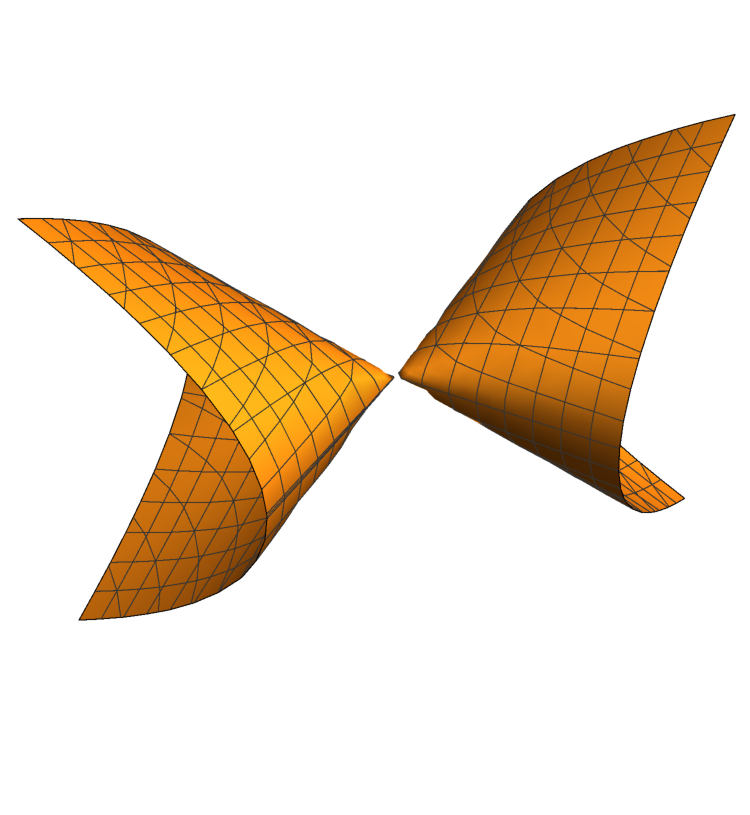
\includegraphics[width = 0.5\textwidth]{cones}
	\caption{Real projection of a quadratic cone.}\label{fig:cone}
\end{figure}

\begin{ex}
	For $C=\mathbb{R}_{\geq 0}({e_1,e_1-2e_2})$, its dual cone $C^\vee=\mathbb{R}_{\geq 0}(2e_1+e_2, -e_2,)$, the semigroup $S_C=C^\vee\cap M$ is generated by minimal integral basis $\{ a_1= e1,a_2=-e_2, a_3=2e_1+e_2\}$. There is a linear relation 
	\begin{equation*}
		a_2+a_3=2a_1,
	\end{equation*}
	thus $z^{a_2}z^{a_3}=z^{2a_1}$ and the corresponding affine toric variety has the following parametrization
	\begin{equation*}
		u_2u_3=u_1^2.
	\end{equation*}
	$U_C$ in this case is a quadratic cone  in Figure~\ref{fig:cone}. It has a singularity at $(0,0,0)\in \mathbb{A}^3$.
\end{ex}
We still need to glue affine toric varieties up to get projective toric varieties. The first step is to glue  cones together.
\begin{dfn}
Let $\Sigma$ be a set of rational polyhedral cones. Then $\Sigma$ is called a \textbf{fan} if 
\begin{itemize}
\item each face of cones in $\Sigma$ is also a cone in $\Sigma$, and
\item the intersection of any two cones in $\Sigma$ is a face of each.
\end{itemize}
\end{dfn}

\begin{dfn}\label{fan} 
Let $\Sigma\subset N_{\mathbb{R}}$ be a fan.
A fan is 
\begin{itemize}
\item
	\textbf{smooth} (or \textbf{regular}) if all the cones in $\Sigma$ are smooth (or \textbf{regular}).
\item
	\textbf{simplicial} if all the cones in $\Sigma$ are simplicial,
\item 
	\textbf{complete} if
	\begin{equation*}
		|\Sigma|=\underset{C\in\Sigma}{\cup}C=N_\mathbb{R},
	\end{equation*}
\end{itemize}
\end{dfn}

Let $\Sigma$ be a fan. We can associate a \textbf{toric variety} $X_\Sigma$ to $\Sigma$. If $C\subset N_\mathbb{R}$ let $C^\vee\subset M_\mathbb{R}$ be the dual cone. Then we have 
\begin{equation*}
S_C=\mathbb{C}[\{z^{m}\}],\  m\in C^\vee\cap M
\end{equation*}
and we let $U_C$ be the affine variety $Spec\ S_C$. The variety $U_C$ is the \textbf{toric chart} associated to $C$.
And then we can glue up all the affine toric varieties with respect to the combinatorics of $\Sigma$ to get the \textbf{toric variety} $X_\Sigma$ associated to the fan. The standard procedure goes as follows.
Consider two cones $C, C'$ and their common face $D:=C\cap C'\in \Sigma$. $D$ is a face of $C$, then, we have $C^\vee\subset D^\vee$ and $\mathbb{C}[{S_C}]\subset \mathbb{C}[{S_D}]$ as a subring. Then by the fact that $Spec: \{Comm\ Rings\}\rightarrow \{Affine\ Schemes\}$ is controvariant functor.

\[ \begin{tikzcd}
\mathbb{C}[S_C] \arrow{r}{\iota} \arrow[swap]{d}{Spec} 
& \mathbb{C}[S_D] \arrow{d}{Spec} \\%
U_C & U_D\arrow{l}{Spec(\iota)}
\end{tikzcd}
\]
Then we can identify $U_{C\cap C'}$ with a principal open subvariety of $U_{C}$ and $U_{C'}$ and glue $U_C$ and $U_C'$ together along $U_{C\cap C'}$. The above procedure also serves as the definition of \textbf{Toric Variety} $X_{\Sigma}$ for a fan $\Sigma$.

\begin{dfn}
	Suppose we have two fans $\Sigma\subset N_{\mathbb{R}}$ and $\Sigma'\subset N'_{\mathbb{R}}$. We define the \textbf{product of fans}
	$$
		\Sigma\times \Sigma':=\{C\times C'|C\in\Sigma,\ C'\in \Sigma'\}.
	$$
	to be a fan in $N_{\mathbb{R}}\times N'_{\mathbb{R}}=(N\times N')_{\mathbb{R}}$
\end{dfn}

\begin{prop}\label{products}
$$
	X_{\Sigma\times \Sigma'}=X_{\Sigma}\times X_{\Sigma'}
$$
\flushright{\qedsymbol}
\end{prop}


Now we will give some concrete examples for both better understanding and latter use.
\begin{ex}\label{Pn}
	(Projective space $\mathbb{P}^n$) The complex projective space $\mathbb{P}^n$ is determined by the fan $\Sigma$ with $n$-dimensional cones
	\begin{equation*}
	\begin{aligned}
		C_0 & :=\mathbb{R}_{\geq 0}(e_1,...e_n),\\
		C_i & :=\mathbb{R}_{\geq 0}(e_1,...e_{i-1},e_{i+1},...,e_n,-(e_1+...+e_n))\ \text{for } i=1,...,n.
	\end{aligned}
	\end{equation*}
	Then we have
	$$
	\begin{aligned}
		U_{C_0} & =Spec(S_{C_0})\cong Spec(\mathbb{C}[u_1,...u_n]),\\
		U_{C_i} & =Spec(S_{C_i})\cong Spec(\mathbb{C}[u_1 u_i^{-1},...u_i^{-1}...u_n u_i^{-1}]) \text{ for } i=1,...n.
	\end{aligned}
	$$
 	The $n+1$ affine toric varieties are just the affine charts used to define projective spaces. From proposition~\ref{products}, we also know that any finite product of projective spaces is a toric variety.
\end{ex}

\begin{ex}
\begin{figure}
	\centering
	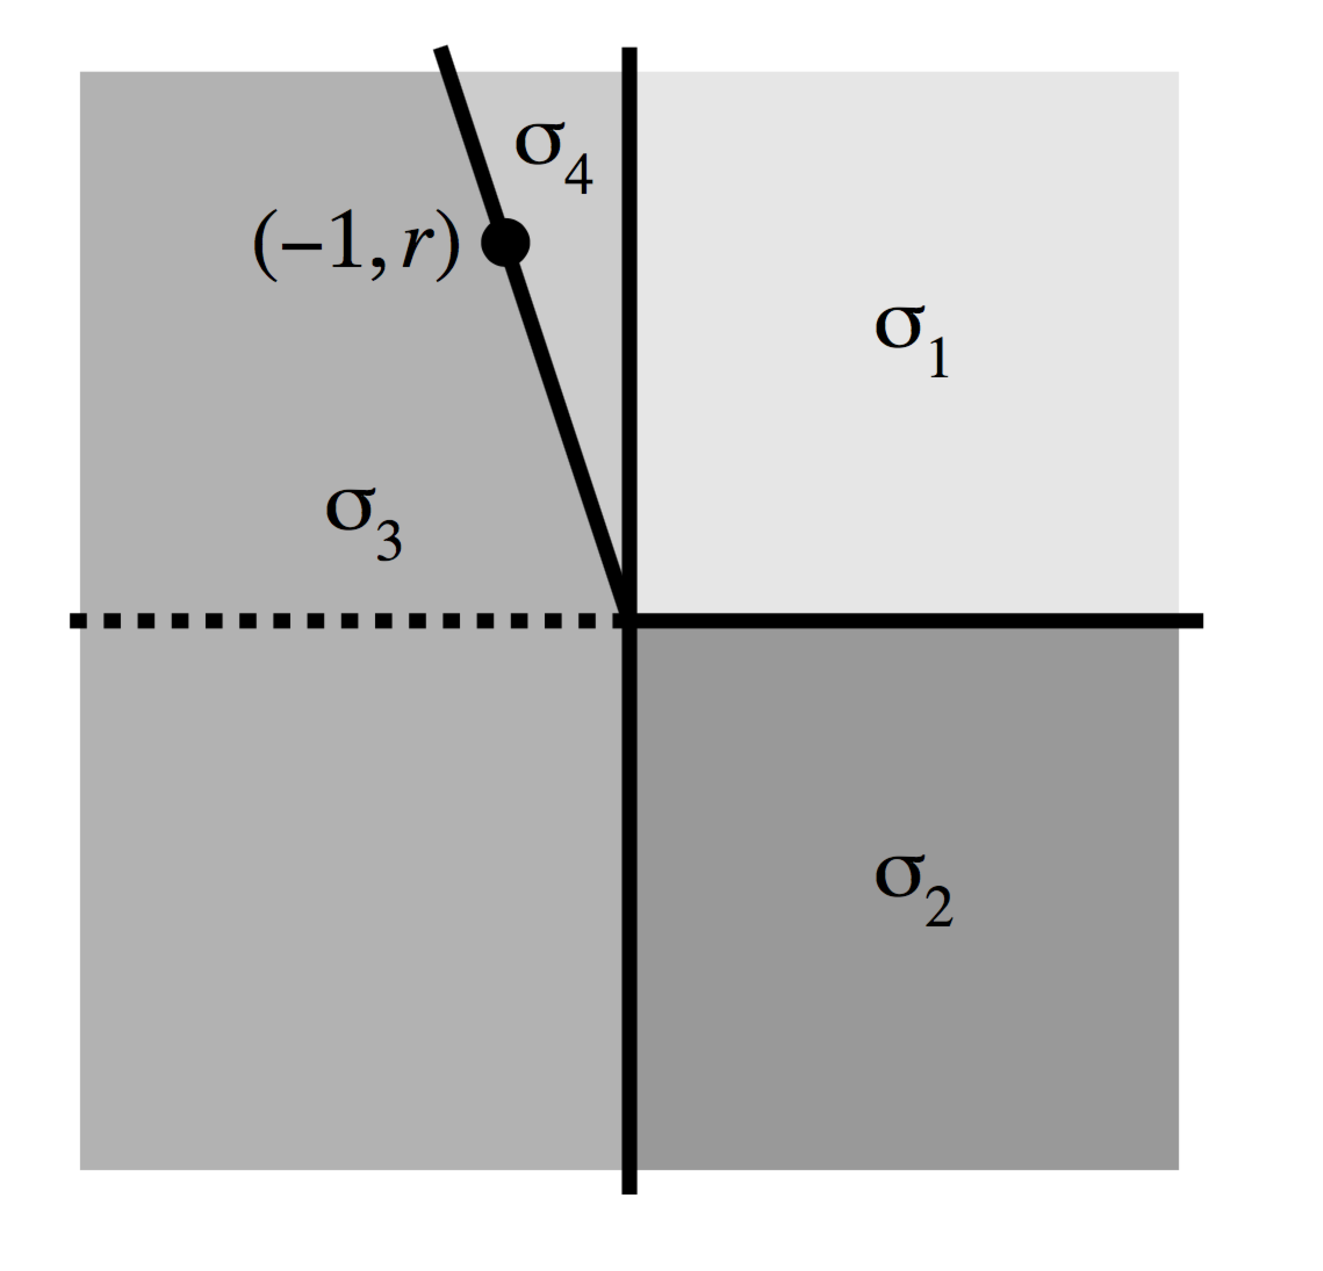
\includegraphics[width = 0.5\textwidth]{Hirzebruch}
	\caption{The fan $\Sigma_r$, and $X_{\Sigma_r}=\mathcal{H}_r$}\label{fig:fan}
\end{figure}
Another set of examples are the Hirzebruch surfaces $\mathcal{H}_r$. Hirzebruch surfaces are hypersurfaces in $\mathbb{P}^1\times \mathbb{P}^2$ with homogeneous coordinates presentation $\{([\eta_0,\eta_1],[\xi_0,\xi_1,\xi_2]),(\eta_0,\eta_1)\neq(0,0),\ (\xi_0,\xi_1,\xi_2)\neq(0,0,0)\}$. The variety is given by the equation
$$
	\eta_0^r\xi_0=\eta_1^r\xi_1,\ \  r\in \mathbb{Z}$$
They correspond to the collection of the fans given in Figure~\ref{fig:fan}
\end{ex}

Now that we have illustrated how to construct toric varieties from fans, one naturally asks how is the geometry and topology of $X_{\Sigma}$ encode the combinatoric data of $\Sigma$. As the name implies, a smooth fan does give rise to a smooth toric variety. 
\begin{thm}
	Let $\Sigma\subset N_{\mathbb{R}}$ be a fan, and $X_{\Sigma}$ be its corresponding toric variety. Then:
	\begin{enumerate}[label=(\alph*)]
		\item $X_\Sigma$ is a smooth variety if and only if the fan $\Sigma$ is smooth.
		\item $X_\Sigma$ is an orbifold ($X_{\Sigma}$ has only finite quotient singularities) if and only if the fan $\Sigma$ is simplicial.
		\item $X_\Sigma$ is compact in ordinary topology if and only if the fan $\Sigma$ is complete.
	\end{enumerate}
\end{thm}
\begin{proof}
For part (a), we only need to verify that a smooth cone gives a smooth affine variety, because smoothness is a local property which has been done in Theorem~\ref{smooth_affine}.
The proof of  part (b) can be found in the Chapter 11 of \cite{cox2009toric}.
For a concise proof of part (c), one refer to Theorem 9.1 of \cite{ewald2012combinatorial}.  
\end{proof}
\subsection{Orbit-Cone Correspondence}
\begin{ex}
	\begin{figure}
	\centering
	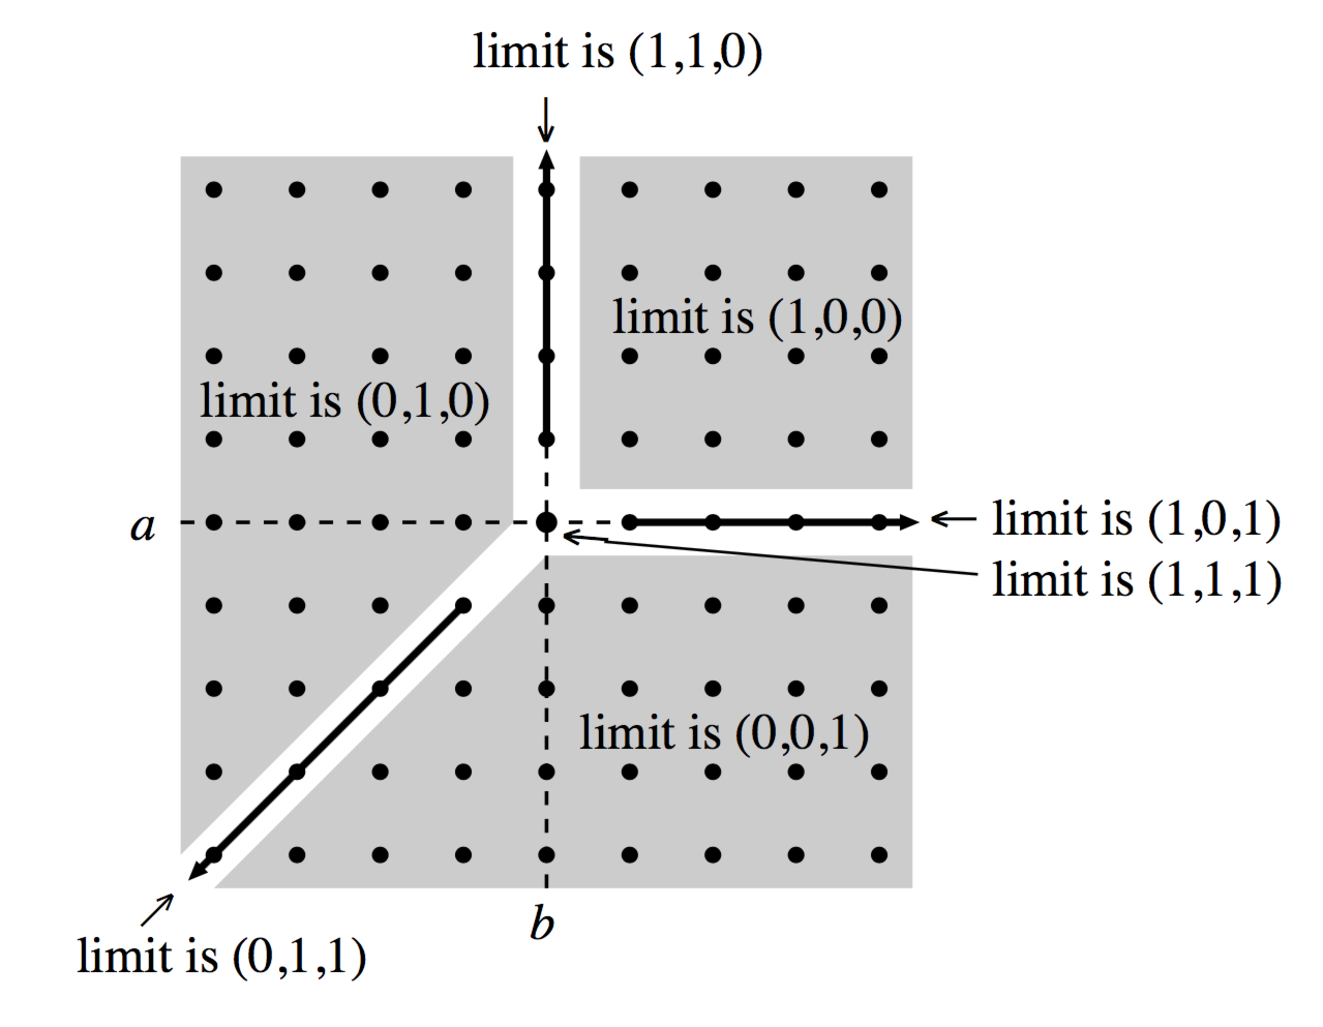
\includegraphics[width = 0.8\textwidth]{limit}
	\caption{limit point corresponding to $(a,b)\in \intg^2$}\label{fig:limit}
\end{figure}
	Consider $\mathbb{P}^2$ for fan in Example~\ref{Pn}. The torus $T_N=(\cplx)^2\subset\mathbb{P}^2$ consists of points with homogeneous coordinates $[1,u,v], u,v\neq0$. Element $(a, b)$ of the lattice $N=\intg^2$ correspond to some one-parameter subgroup of $T_N$ via the the map

	\[ \begin{tikzcd}
	\cplx^* \arrow{r}{\lambda^{(a,b)}} & (\cplx^*)^2 \arrow{r} & \mathbb{P}^2\\%
	t \arrow[r,mapsto]		& (t^a, t^b) & \\
	\ & (u,v)\arrow[r] & \ [1,u,v]
	\end{tikzcd}\]	
	Observe that, suppose $a,b>0,$
		\begin{equation*}
			\lim_{t\rightarrow0} \lambda^{(a,b)}(u)=\lim_{t\rightarrow0}[1, t^a,t^b]=[1,0,0].
		\end{equation*}
		Notice we are using the homogeneous coordinates.
		For the case $b>a,\ a<0,$ $\lim_{t\rightarrow0}[1,t^a,t^b]=\lim_{t\rightarrow 0}[t^{-a},1,t^{a-b}]=[0,1,0]$
	The Figure~\ref{fig:limit} illustrates the pattern how the limit point in $\mathbb{P}^2$ relies on $(a,b)$. And we observe that regions corresponding to different limit points are just the cones of the fan $\Sigma$.
\end{ex}
With the heuristic example above, we state the following theorem
\begin{thm}\label{corre}
Let $\Sigma\subset N_\reals$ be a fan and $X_{\Sigma}$ be the corresponding toric variety.
\begin{enumerate}[label=(\alph*)]
\item There is a bijective correspondence
	\[ \begin{tikzcd}
	\{\text{Cones }C\in \Sigma\}\arrow{r} & \{T_{N}\text{-orbits in }X_{\Sigma}\} \\
	C \arrow[r,mapsto]		& O(C). \\
	\end{tikzcd}\]
\item The correspondence satisfies the relation
	\begin{equation*}
		\text{dim } O(C)=\text{dim }N_{\reals}-\text{dim} C.
	\end{equation*}
\item If we take orbit closure, then the correspondence reverse the inclusion relation, i.e.,
	\begin{equation*}
		C\subset C'\Leftrightarrow \overline{O(C)}\supset \overline{O(C')}
	\end{equation*}
\end{enumerate}
\end{thm}
Specially, the set of one dimensional cones $\Sigma(1)\in \Sigma$ corresponds to torus invariant subvarieties of codimension 1 in $X_\Sigma$, and the top dimensional cones $\Sigma(n)\in\Sigma$ corresponds to the fixed point of the torus action in $X_\Sigma$.

\subsection{Divisor, Cohomology on Toric Variety}
Firstly, we have to recall some basic notions in algebraic geometry.
\begin{dfn}
	Let $X$ be an irreducible variety. An irreducible subvariety of codimension one in $X$ is called a \textbf{prime divisor}. Denote the free abelian group generated by prime divisors on $X$ by $\text{Div}(X)$. An element $\sum_D n_D D$ of $\text{Div}(X)$ is a \textbf{Weil Divisor} if the collection $\{D|n_D\neq 0\}$ is locally finite. A Weil divisor $D$ is \textbf{effective} if the coefficients re non-negative and $D>D'$ if $D-D'$ is effective. 
\end{dfn}

\begin{dfn}
	Let X be normal variety. 
	\begin{enumerate}[label=(\alph*)]
	\item The divisor of a nonzero function $f\in \cplx(X)^*$ is 
		\begin{equation*}
			div(f):=\sum_D v_D(f) D,
		\end{equation*}
		where the sum is over all the prime divisors in $X$, and $v_{D}(f)$ is the order of vanishing of $f$ along $D$. 
	\item It can be shown that $\{D|v_D(f)\neq0\}$ is locally finite. Divisors of this form are called \textbf{Principal Weil Divisors} and the set of all principal Weil Divisors is denoted $\text{Div}_0(X)$. The definition of $v_D$ can be found at pp 264 of \cite{ewald2012combinatorial}.
	\item A Weil divisor $D$ on a X is \textbf{Cartier} if it is \textbf{locally principal}, which means that there exist a collection of $\{(U_i, f_u)\}_{i\in I}$ such that $D|_{U_i}=\text{div}(f_i)|_{U_i}$. Denote the set of Cartier divisors as $\text{CDiv}(X)$
	\end{enumerate}
\end{dfn}
Obviously, we have
\begin{equation*}
	\text{Div}_0(X)\subset \text{CDiv}(X)\subset\text{Div}(X).
\end{equation*}
Then we have the following group of equivalence classes
\begin{dfn}
	$X$ is a normal variety. Its \textbf{class group} is
	\begin{equation*}
		\text{Cl}(X):=\text{Div}(X)/\text{Div}_0(X),
	\end{equation*}
	and its \textbf{Picard group} is 
	\begin{equation*}
		\text{Pic}(X):=\text{CDiv}(X)/\text{Div}_0(X).
	\end{equation*}
\end{dfn}
Divisors are naturally related to sheaves and line bundles on normal varieties, and the Picard group is just the group of linear equivalent class line bundles. Recall that the structure sheaf $\calo_X$ of $X$ could be defined by
\begin{equation*}
	U\mapsto\calo_X(U)=\{f\in \cplx(X)^*|div(f)|_U\geq0\}\cup\{0\}.
\end{equation*}
Similarly, we define for the sheaf $\calo_X(D)$ for divisor $D$.
\begin{dfn}
$D$ is a Weil divisor on a normal variety $X$. Then $\calo_X(D)$ is a sheaf of $\calo_X$-module defined by
\begin{equation*}
	U\mapsto\calo_X(D)(U):=\{f\in \cplx(X)^*|(\text{div}(f)+D)|_U\geq0\}\cup\{0\}.
\end{equation*}
\end{dfn}
\begin{prop}
For a Weil divisor, the sheaf $\calo_X(D)$ defined above is a coherent sheaf of $\calo_X$-module on $X$. Furthermore, when $D$ is a Cartier divisor, $\calo_X(D)$ is the sheaf of sections of a line bundle on $X$.
For a proof, refer to Proposition 4.0.27 and Theorem 6.0.18 in \cite{cox2009toric}. 
\begin{flushright}
	\qedsymbol
\end{flushright}
\end{prop}

\begin{dfn}

	Let $X$ be a nonsingular variety. An \textbf{algebraic $k$-cycle} means a finite linear combination of $k$-dimensional subvarieties of X with integer coefficients. The group is denoted by $Z_k(X)$. A $k$-cycle $\alpha$ is \textbf{rationally equivalent} to 0 if there are finitely many $(k+1)$-dimensional irreducible subvarieties $W_i\subset X$ and nonzero rational functions $f_i\in\cplx(W_i)$ such that
	\begin{equation*}
	\alpha=\sum_i \text{div}_{W_i}(f_i).
	\end{equation*}
	The cycles rationally equivalent to zero form a subgroup $Rat_k(X)$ of $Z_k(X)$. This gives a quotient group
	\begin{equation*}
		A_k(X):=Z_k(X)/Rat_k(X).
	\end{equation*}
	We define the \textbf{Chow group} to be the group of codimension k modulo rational equivalence, denoted by $A^k(X):=A_{n-k}(X)$.
\end{dfn}
For example, when $X$ is a variety of dimension n, the $A^1$ is the divisor class group of $X$. When $X$ is smooth, this is isomorphic to the Picard group.

In the case where $X$ is smooth and projective, it can be shown that graded ring structure exists, with the product
\begin{equation*}
	A^k(X)\times A^{l}(X)\rightarrow A^{k+l}(X)
\end{equation*}
identified with the geometric intersection of cycles in the case of of transverse intersections. We call the graded ring $A^{\bullet}(X)=\oplus_k A^k(X)$ \textbf{Chow ring}. A cycle $\alpha$ in $A^k(X)$ gives a homology class in $H_{2n-2k}(X)$ which is dual to a cohomology class in $H^{2k}(X)$. The intersection of cycles corresponds to cup product in cohomology, so there is a ring homomorphism
\begin{equation*}
	A^\bullet(X)\rightarrow H^\bullet(X).
\end{equation*}
All the above notions are introduced in general varieties. The detailed construction require some elaborated knowledge of intersection theory (see Chapter 8 of \cite{fulton2013intersection}), which we only give a sketch here.

In the context of toric varieties, however, with the torus action, the statement are generally stronger and usually directly related with the combinatoric data.

Let $X_\Sigma$ be toric variety of a fan $\Sigma$ in $N_\reals$ with $\text{dim } N_\reals=n$. By the Orbit-Cone correspondence (Theorem~\ref{corre}), $k$-dimensional cones $C\in \Sigma$ corresponds to a $(n-k)$-dimensional $T_N$-orbit in $X_\Sigma$. Let $\Sigma(1)$ denote the set of one-dimensional cones in $\Sigma$. For each $\rho\in \Sigma(1)$ there is a $T_N$-invariant divisor $D_{\rho}:=\overline{O(\rho)}\subset X_\Sigma$. By Poincare duality, there is a cohomology class associated to $[D_\rho]$ in $H^2(X_\Sigma)$. When $X_\Sigma$ is nonsingular, the cohomology class $[D_\rho]$ generate the cohomology ring $H^*(X_\Sigma, \mathbb{Z})$ as follows.

\begin{dfn}\label{ideals}
Let $X_\Sigma$ be a complete simplicial toric variety and fix a numbering $\rho_1,...,\rho_r$ for the rays in $\Sigma(1)$. Also let $u_i$ be the minimal generator of $\rho_i$ and introduce a variable $x_i$ for each $\rho_i$. In the ring $\mathbb{Z}[x_1,...,x_r]$, let $\mathcal{I}$ be the monomial ideal with square-free generators as follows:
\begin{equation*}
\mathcal{I} = \langle x_{i_1}\cdot\cdot\cdot x_{i_s} | i_j \text{ are distinct and } \rho_{i_1}+...+\rho_{i_s} \text{ is not a cone of } \Sigma\rangle.
\end{equation*}
We call $\mathcal{I}$ the \textbf{Stanley-Reisner ideal}. Also, we let $\mathcal{J}$ be the ideal generated by the linear forms
\begin{equation*}
\sum_{i}^r\langle m, u_i \rangle x_i 
\end{equation*}
where $m$ ranges over $M$ (or equivalently, over some basis for $M$).
\end{dfn}
With these two ideal defined, we get the combinatoric presentation of the cohomology ring.
\begin{thm}
(Jurkiewicz-Danilov, Theorem 12.4.4 of \cite{cox2009toric}) Let $X_\Sigma$ be a smooth complete toric variety. For the polynomial ring $\intg[x_1,...,x_r]$ indexed by $\rho_1,..,\rho_r\in \Sigma(1)$, let $\mathcal{I}$ and $\mathcal{J}$ be the ideals in Definition~\ref{ideals} and define
\begin{equation*}
R[\Sigma]:=\mathbb{Z}[x_1,...,x_K]/{(\mathcal{I}+\mathcal{J})}.
\end{equation*}
Then the following holds:

	\[ \begin{tikzcd}
	R[\Sigma] \arrow[r,equal] & A^\bullet(X_\Sigma) \arrow[r,equal] & H^\bullet(X_\Sigma)\\%
	x_i \arrow[r,mapsto]		& D_{\rho_i} & \\
	\ & D_{\rho_i}\arrow[r,mapsto] & \ [D_{\rho_i}]
	\end{tikzcd}\]	
It follows that $H^{odd}(X_\Sigma,\mathbb{Z})=0$, and $H^{2i}(X_\Sigma,\intg)\cong A^i(X_\Sigma)$ and in particular, $H^2(X_\Sigma,\intg)\cong Pic(X_\Sigma)$.
\end{thm}

\section{Main Results}
From now on, we will abuse the notation to write $D_\rho$ instead of $[D_\rho]$ as the cohomology classes and divisor classes. We consider a smooth compact toric variety $X:=X_\Sigma$ corresponding to $\Sigma\in N_\reals$, where $N$ is a lattice of dimension $n$ and $M$ being its dual lattice. Let $\Sigma(1)$ denote the set of one dimensional cones in $\Sigma$ and assume that $|\Sigma(1)|=r$ a By Proposition 4.2.1 and 4.2.5 in \cite{cox2009toric}, we know $\text{Pic}(X_\Sigma)$ is torsion-free and
\begin{equation*}
0\longrightarrow M\longrightarrow \intg^r\longrightarrow \text{Pic}(X_\Sigma)\longrightarrow 0.
\end{equation*}
If we set the Picard number $k$, we have the relation
\begin{equation*}
	\text{dim }X =\text{dim }N=n=r-k.
\end{equation*}
After we quotient the ideal generated by the linear relations, we can equivalently say that the cohomology ring is multiplicatively generated by a basis of the Picard group. We denote the basis of Picard group as $q_1,...q_k$, and express the invariant divisor as
\begin{equation*}
D_{\rho_i}=\left\{
\begin{aligned}
& q_i & 1\leq i\leq k\\
& \sum_{j=1}^k m_{i j} q_j  &k+1\leq i\leq r
\end{aligned}
\right.
\end{equation*}
Then let's consider a smooth complete intersection $Y$ as a generic intersection of $s$ hypersurfaces $\{Y_l\}_{1\leq l\leq s}$. Each $Y_l$ is dual to the cohomology class $\sum_{j}^k d_{l j} q_j$. In the context of smooth manifold, by the transversality argument, one can always deform the hypersurfaces (not algebraic now) so that they intersects transversally. Thus $Y$ is submanifold of complex dimension $r-k-s$. In this section we will consider the Witten genus on $Y$.
\subsection{Witten Genus on Toric Complete Intersections}
The exact sequence 
\begin{equation*}
0\longrightarrow \Omega_{\mathbb{P}^n}^{1}\longrightarrow\mathcal{O}_{\mathbb{P}^n}(-1)^{n+1}\longrightarrow \mathcal{O}_{\mathbb{P}^n} \longrightarrow0,
\end{equation*} called \textbf{Euler sequence of }$\mathbb{P}^n$ is of fundamental importance because the it links the cotangent bundle with the canonical line bundles on $\mathbb{P}^n$. For smooth toric varieties, there is a \textbf{generalized Euler sequence}( see Theorem 8.1.6 in \cite{cox2009toric}).
\begin{equation*}
0\longrightarrow \Omega_{X_\Sigma}^1\longrightarrow \oplus_{\rho\in \Sigma(1)}\mathcal{O}_{X_\Sigma}(-D_\rho)^{n+1}\longrightarrow \text{Pic}(X_\Sigma)\otimes_\intg \mathcal{O}_{X_\Sigma} \longrightarrow0.
\end{equation*}
Take the dual of the above exact sequence, we get 
\begin{equation*}
0\longrightarrow \mathcal{O}_{X_\Sigma}^{\oplus k}\longrightarrow\oplus_{\rho\in \Sigma(1)}\mathcal{O}_{X_\Sigma}(D_\rho)\longrightarrow TX_{\Sigma}\longrightarrow0,
\end{equation*}
where $k$ is the rank of $\text{Pic}(X_\Sigma)$ or equivalently the rank of $H^2(X_\Sigma,\mathbb{Z})$.
from which we can calculate the total Chern class and all the multiplicative genera of $TX_{\Sigma}$. 

The $\mathcal{O}_{X_\Sigma}(D_\rho)$ is the line bundle defined by the divisor $D_\rho$ in the Picard group, of which the first Chern class is $D_\rho\in H^2(X_\Sigma,\intg)$.
Then by the multiplicative property of total Chern class, we have
\begin{equation*}
	c(TX)=\oplus_{\rho\in\Sigma(1)}\  c(\mathcal{O}_{X_\Sigma}(D_\rho))=\prod_{\rho\in \Sigma(1)}(1+D_\rho).
\end{equation*}
The $\{D_\rho\}$ play the role of Chern roots here, which is not coincidence.
For a general multiplicative genus $\varphi_Q$ corresponding to even power series $Q(x)$, we observe that
\begin{equation*}
\varphi_Q(TX)=\frac{\varphi_Q\left(\bigoplus_{\rho\in \Sigma(1)}\mathcal{O}(D_\rho)\right)}{\varphi_Q(\mathcal{O}(X_\Sigma)^{\oplus k})}=\frac{\prod_{\rho\in \Sigma(1)} Q(D_\rho)}{Q(0)^k},
\end{equation*}
In the case of Witten genus, we have
\begin{equation*}
\begin{aligned}
\mathcal{W}(T_\reals X)&=\prod_{\rho\in \Sigma(1)}D_\rho \frac{\theta'(0,\tau)}{\theta(D_\rho,\tau)},\\
W(X_\Sigma)&=\left\langle\mathcal{W}(X_\Sigma),[X_\Sigma]\right\rangle
\end{aligned}
\end{equation*}
Consider the inclusion map $\iota: Y\rightarrow X_\Sigma$, we have the adjunction formula:
$$
0\longrightarrow TY\longrightarrow\iota^*TX_{\Sigma}\longrightarrow\iota^* N_X Y\longrightarrow0,
$$
where the normal bundle $N_X Y$ is isomorphic to $\bigoplus_{l=1}^s\mathcal{O}(\sum_{j}^k d_{l j} q_j)$.
By the multiplicative properties of Chern class, we have the following data:
\begin{equation*}
c(TY)=\iota^*\left(\frac{c(TX)}{c(N_X Y)}\right)=\iota^*\left(\frac{\prod_{i=1}^k (1+q_i)\prod_{j=k+1}^{r}(1+\sum_{i=1}^k m_{ji}q_i)}{\prod_{l=1}^s(1+\sum_{j}^k d_{l j} q_j)}\right).
\end{equation*}
Following these we have
$$
\begin{aligned}
w_2(T_\mathbb{R}Y)& \equiv c_1(TY) (\text{mod } 2)\\
& =\iota^*\left(\sum_{i=1}^k q_i+\sum_{j=k+1}^{r} \sum_{i=1}^k m_{ji}q_i-\sum_{l=1}^s\sum_{i=1}^k d_{l i}q_i\right) \text{     (mod } 2)
\end{aligned}
$$
and 
$$
p_1(T_{\mathbb{R}}Y)=\iota^*\left(\sum_{i=1}^k q_i^2+\sum_{j=k+1}^r (\sum_{i=1}^k m_{ji}q_i)^2-\sum_{l=1}^s(\sum_{i=1}^k d_{l i}q_i)^2\right).
$$
Because we know little about the $H^4(X,\intg)$, it is difficult to tell whether the above presentation of Pontryagin class vanishes in the general case. Still, we know the complete intersection is string when all the coefficients of $\{q_i q_j\}$ vanishes. On the other hand, because of the multiplicative property of Witten class, we have
\begin{equation*}
\begin{aligned}
\mathcal{W}(T_\reals Y)
&=\iota^*\left(\frac{\mathcal{W}(T_\reals X)}{\mathcal{W}((N_X Y)_\reals)}\right)\\
&=\iota^*\left(\frac{\prod_{i=1}^k q_i \frac{\theta'(0,\tau)}{\theta(q_i,\tau)}\prod_{j=k+1}^r (\sum_{t=1}^k m_{j t}q_t) \frac{\theta'(0,\tau)}{\theta(\sum_{t=1}^k m_{jt}q_t,\tau)}}{\prod_{l=1}^s(\sum_{j=1}^k d_{l j} q_j) \frac{\theta'(0,\tau)}{\theta(\sum_{j=1}^k d_{l j} q_j,\tau)}}\right).
\end{aligned}
\end{equation*}
Integrate the above formula over the fundamental class of Y, we have
$$
\begin{aligned}
\int_{Y} \mathcal{W}(T_\reals Y) 
& =\int_X \iota_!\iota^*\left(\frac{\mathcal{W}(T_\reals X)}{\mathcal{W}((N_X Y)_\reals)}\right)\\
& =\int_X \left(\frac{\mathcal{W}(T_\reals X)}{\mathcal{W}((N_X Y)_\reals))}\right)\smile e(N_X Y)\\
& =\int_X \left(\frac{\prod_{i=1}^k q_i \frac{\theta(q_i,\tau)}{\theta'(0,\tau)}\prod_{j=k+1}^r (\sum_{t=1}^k m_{j t}q_t) \frac{\theta(\sum_{t=1}^k m_{jt}q_t,\tau)}{\theta'(0,\tau)}}{\prod_{l=1}^s(\sum_{j=1}^k d_{l j} q_j) \frac{\theta(\sum_{j=1}^k d_{l j} q_j,\tau)}{\theta'(0,\tau)}}\right)\cdot \prod_{l=1}^s(\sum_{j=1}^k d_{l j} q_j)\\
& =\int_X \left(\frac{\prod_{i=1}^k q_i \frac{\theta(q_i,\tau)}{\theta'(0,\tau)}\prod_{j=k+1}^r (\sum_{t=1}^k m_{jt}q_t) \frac{\theta(\sum_{t=1}^k m_{jt}q_t,\tau)}{\theta'(0,\tau)}}{\prod_{l=1}^s \frac{\theta(\sum_{j=1}^k d_{l j} q_j,\tau)}{\theta'(0,\tau)}}\right),
\end{aligned}
$$
where $e(N_x Y)$ in the second line is the Euler class of the normal bundle.
\subsection{Equivariant Localization and Genera as Residues}
In this section, we further restrict our setting to $n$-dimensional smooth compact symplectic toric variety $X$ of Picard number $k$, for which the fan $\Sigma$ is the normal fan of a Delzant polytope \cite{da2001symplectic}. For $|\Sigma(1)|=r=n+k$, they are equipped with an action of rank $r$ compact torus $T$ with $|\Sigma(n)|$ isolated fixed points.
 
Let's now have a brief recall on the construction of equivariant cohomology over toric varieties. Let $G$ be a compact connected Lie group, classified by  the principal $G$-bundle $EG\rightarrow BG$, whose total space is contractible. This bundle is uniquely determined up to homotopy equivalence. Then $G$ acts on the the space$X\times EG$ freely. We consider the famous \textbf{Borel's Construction} \cite{borel1960seminar}
\begin{equation}
	X\times_G EG=(X\times EG)/G.
\end{equation}
And the \text{equivariant cohomology} of $X$ is defined to be 
\begin{equation}
	H^\bullet_{G}(X)=H^\bullet(X\times_G EG).
\end{equation}
Then, in the case of our setting, we choose the torus $T$ to be the lie group. Note that 
$$
H^\bullet_T(\{pt\},\ratl)=H^\bullet(BT,\ratl)=H^\bullet((\mathbb{CP^\infty})^r,\ratl)=\mathbb{Q}[\lambda_1,\lambda_2,...,\lambda_r ],
$$
and each $\lambda_i$ has degree 2.

There is a ring morphism between the ordinary cohomology ring $H^\bullet(X,\mathbb{Q})$ and the equivariant cohomology ring $H_{T}^{\bullet}(X,\mathbb{Q})$. $H^\bullet_T(X_\Sigma)$ can be thout of as an $H^\bullet(BT)$-module. Note also that the inclusion of a fiber $i_{X}: X_\Sigma\rightarrow X\times_G EG$ induces the ``Non-equivariant limit'' map $i^*_X: H^\bullet_T(X_\Sigma)\rightarrow H^\bullet(X_\Sigma)$, which amounts to mapping all $\lambda_i$ to 0.
\begin{prop}
Every $D_\rho$ has an equivariant counterpart $(D_\rho)_T$, where $\rho\in \Sigma(1)$. This map induces the morphism between cohomology and their equivariant counterpart.
\begin{equation*}
\begin{aligned}
D_\rho & \longrightarrow (D_{\rho})_T=D_\rho-\lambda_\rho\in H^2_T(X,\ratl)\\
 H^\bullet (X,\ratl)&\longrightarrow H^\bullet_T(X_\Sigma,\mathbb{Q})=\mathbb{Q}[(D_{\rho_1})_T,...,(D_{\rho_r})_T]/(\mathcal{I}_T+\mathcal{J}_T)\\
\end{aligned}
\end{equation*}
where
\begin{equation*}
\mathcal{I}_T = \langle (D_{i_1})_T\cdot\cdot\cdot (D_{i_s})_T | i_j \text{ are distinct and } \rho_{i_1}+...+\rho_{i_s} \text{ is not a cone of } \Sigma\rangle
\end{equation*}
and $\mathcal{J}_T$ is the ideal generated by the linear forms
\begin{equation*}
\sum_{i}^r\langle m, u_i \rangle (D_{\rho_i})_T
\end{equation*}
where $m$ ranges over $M$ (or equivalently, over some basis for $M$).

\end{prop}
\begin{proof}
Proposition 12.4.13 in \cite{cox2009toric} and \cite{givental1998mirror},
\end{proof}

Following Givental \cite{givental1998mirror}, we can find an explicit way to proceed calculations via the Atiyah-Bott localization.
\begin{thm}
$f(q_1,...,q_k,\{\lambda_i\})$ is a polynomial in $H^\bullet_T(X,\ratl)$, integrating it over the fundamental class $[X]$ maps it into $\ratl[\lambda_1,...,\lambda_r]$. Explicitly, we have
\begin{equation}\label{localization}
\int_{X} f(q_1,...,q_k,\{\lambda_i\})=\sum_\alpha Res_\alpha \frac{f(q_1,...,q_k,\{\lambda_i\})}{(D_1)_T\cdot (D_2)_T\cdot ...\cdot (D_r)_T} d q_1 dq_2...dq_k
\end{equation}
\end{thm}
\begin{proof}
This equation can be proved via Atiyah-bott localization and arguments can be  found at pp 22 of \cite{givental1998mirror}. 
\end{proof}
If we take the non-equivariant limit we can get an explicit formula to calculate the the integration of $f(p,0)$ over the fundamental class $[X]$.
\subsection{Vanishing result for some string complete intersection}
What we want to calculate is
\begin{equation*}
\begin{aligned}
\int_{Y} \mathcal{W}(T_\reals Y) 
& =\int_X \iota_!\iota^*\left(\frac{\mathcal{W}(T_\reals X)}{\mathcal{W}((N_X Y)_\reals)}\right)\\
& =\int_X \left(\frac{\prod_{i=1}^k q_i \frac{\theta'(0,\tau)}{\theta(q_i,\tau)}\prod_{j=k+1}^r (\sum_{t=1}^k m_{jt}q_t) \frac{\theta'(0,\tau)}{\theta(\sum_{t=1}^k m_{jt}q_t,\tau)}}{\prod_{l=1}^s \frac{\theta'(0,\tau)}{\theta(\sum_{j=1}^k d_{l j} q_j,\tau)}}\right).
\end{aligned}
\end{equation*}
With the localization argument before, we can consider a integral of polynomial $\mathcal{W}(q,\{\lambda_i\})$ in $H^\bullet_T(X,\ratl)$ which under nonequivariant limit gives the integral we want. The choice is not unique. We can choose

\begin{equation*}
\begin{aligned}
\int_{Y} \mathcal{W}(T_\reals Y) 
& =i_X^*\int_X \left(\frac{\prod_{i=1}^k (q_i-\lambda_i) \frac{\theta'(0,\tau)}{\theta(q_i-\lambda_i,\tau)}\prod_{j=k+1}^r (\sum_{t=1}^k m_{jt}q_t-\lambda_j) \frac{\theta'(0,\tau)}{\theta(\sum_{t=1}^k m_{jt}q_t-\lambda_j,\tau)}}{\prod_{l=1}^s \frac{\theta'(0,\tau)}{\theta(\sum_{j=1}^k d_{l j} q_j,\tau)}}\right)\\
\end{aligned}
\end{equation*}
By Eq.~\ref{localization},
\begin{equation*}
\begin{aligned}
&\int_{Y} \mathcal{W}(T_\reals Y) \\
& =i_X^*\sum_\alpha res_\alpha \frac{\left(\frac{\prod_{i=1}^k (q_i-\lambda_i) \frac{\theta'(0,\tau)}{\theta(q_i-\lambda_i,\tau)}\prod_{j=k+1}^r (\sum_{t=1}^k m_{jt}q_t-\lambda_j) \frac{\theta'(0,\tau)}{\theta(\sum_{t=1}^k m_{jt}q_t-\lambda_j,\tau)}}{\prod_{l=1}^s \frac{\theta'(0,\tau)}{\theta(\sum_{j=1}^k d_{l j} q_j,\tau)}}\right)}{\prod_{i=1}^k (q_i-\lambda_i)\prod_{j=k+1}^r (\sum_{t=1}^k m_{jt}q_t-\lambda_j)}\\
& =i_X^*\sum_\alpha res_\alpha\left(\frac{\prod_{l=1}^s \frac{\theta(\sum_{j=1}^k d_{l j} q_j,\tau)}{\theta'(0,\tau)}}{\prod_{i=1}^k  \frac{\theta(q_i-\lambda_i,\tau)}{\theta'(0,\tau)}\prod_{j=k+1}^r  \frac{\theta(\sum_{t=1}^k m_{jt}q_t-\lambda_j,\tau)}{\theta'(0,\tau)}}\right)dq_1...dq_k\\
&=\lim_{\lambda_i\rightarrow0}\sum_\alpha res_\alpha \frac{g(q,\tau)}{\prod_{j=1}^r f_j (q,\tau,\{\lambda_i\})}dq_1...dq_k,
\end{aligned}
\end{equation*}
where
\begin{equation*}
\begin{aligned}
g(q_1,..,q_k,\tau)=\prod_{l=1}^s\frac{\theta(\sum_{j=1}^k d_{l j} q_j,\tau)}{\theta'(0,\tau)}
\end{aligned}
\end{equation*}
and
\begin{equation*}
f_j(q_1,...,q_k,\tau,\{\lambda_i\})=\left\{
\begin{aligned}
&\frac{\theta(q_j-\lambda_j,\tau)}{\theta'(0,\tau)} & \text{ for } 1\leq j\leq k\\
& \frac{\theta(\sum_{t=1}^k m_{jt}q_t-\lambda_j,\tau)}{\theta'(0,\tau)} &\text{for } k+1\leq j\leq r
\end{aligned}
 \right.
\end{equation*}
Let's analyze how $g$ and $f$ transform under the translation over the lattice $\{\intg+\intg \tau\}$. By the transforming laws of theta functions[\ref{theta}], without loss of generality, $q_1\rightarrow q_1+1$.
\begin{equation*}
	g(q_1+1,...,q_k,\tau)=(-1)^{d_{11}+...+d_{s1}}g(q_1,...,q_k,\tau),
\end{equation*}
\begin{equation*}
f_j(q_1+1,...,q_k,\tau,\{\lambda_i\})=\left\{
\begin{aligned}
	& - f_1(q_1,...,q_k,\tau,\{\lambda_i\})&\text{for $j=1$}\\
	& f_j(q_1,...,q_k,\tau,\{\lambda_i\})&\text{for $j \neq 1$ and $j\leq k$} \\
	& (-1)^{m_{j1}} f_j (q_1,...,q_k,\tau,\{\lambda_i\})&\text{for $k+1\leq j\leq r$}
\end{aligned}
\right.
\end{equation*}
Then,
\begin{equation*}
\frac{g(q_1,...,q_i+1,...,q_k,\tau)}{\prod_{j=1}^r f_j (q_1,...,q_i+1,...,q_k,\tau,\{\lambda_i\})}=(-1)^{\sum_{j=1}^s d_{ji}-\sum_{j=k+1}^r m_{ji}-1}\frac{g(q,\tau)}{\prod_{j=1}^r f_j (q,\tau,\{\lambda_i\})}.
\end{equation*}
On the other hand under the translation $q_1\rightarrow q_1+\tau$, we have
\begin{equation*}
g(q_1+\tau,...,q_k,\tau)
=(-1)^{d_{11}+...,d_{s1}} e^{-2\pi i\sum_{l=1}^s d_{l1}(\sum^k_j d_{lj}q_j)-\pi i\sum_{l=1}^s d^2_{l1}\tau} g(q_1,...,q_k,\tau),
\end{equation*}
and
\begin{equation*}
\begin{aligned}
&f_j(q_1+\tau,...,q_k,\tau,\{\lambda_i\})=\\
&\left\{
\begin{aligned}
&(-1)e^{-2\pi i (q_1-\lambda_1)-\pi i \tau} f_1(q,\tau,\{\lambda_i\}) &\text{ for $j=1$ }\\
&f_j(q,\tau,\{\lambda_i\}) &\text{ for $i\neq 1$ and $j\leq k$}\\
& (-1)^{m_{j1}} e^{-2\pi i m_{j1}(\sum^k_t m_{jt}q_t-\lambda_j)-\pi i m_{j1}^2 \tau}f_j(q,\tau,\{\lambda_i\})&\text{$k+1 \leq j\leq r$}
\end{aligned}
\right.
\end{aligned}
\end{equation*}
Then the we have the transforming law
\begin{equation*}
\begin{aligned}
&\frac{g(q_1,...,q_i+\tau,...,q_k,\tau)}{\prod_{j=1}^r f_j (q_1,...,q_i+\tau...,q_k,\tau,\{\lambda_i\})}\\
&=(-1)^{\sum_{t=1}^s d_{ti}-\sum_{t=k+1}^r m_{ti}-1}\\
&\times e^{-2\pi \sqrt{-1}[\sum_{v\neq i}^k(\sum_{t}^s d_{t i} d_{tv}-\sum_{u=k+1}^r m_{u i} m_{uv})q_v+(\sum_{t=1}^s d_{ti}^2-\sum^r_{u=k+1}m_{ui}^2-1)q_i-\lambda_i+\sum_{u=k+1}^r m_{ui}\lambda_u]}\\
&\times e^{-\pi \sqrt{-1}(\sum_{t=1}^s d_{ti}^2-\sum^r_{u=k+1}m_{ui}^2-1)\tau}\\
&\times \frac{g(q_1,...,q_i,...,q_k,\tau)}{\prod_{j=1}^r f_j (q_1,...,q_i...,q_k,\tau,\{\lambda_i\})}
\end{aligned}.
\end{equation*}
Remember that
\begin{equation*}
\begin{aligned}
w_2(T_\mathbb{R}Y)& \equiv c_1(TY) (\text{mod } 2)\\
& =\iota^*\left(\sum_{i=1}^k q_i(1+\sum_{j=k+1}^{r} m_{ji}-\sum_{l}^s d_{l i})\right) \text{     (mod } 2),
\end{aligned}
\end{equation*}
and
\begin{equation*}
\begin{aligned}
p_1(T_{\mathbb{R}}Y)&=\iota^*\left(\sum_{i=1}^k q_i^2+\sum_{j=k+1}^r (\sum_{i=1}^k m_{ji}q_i)^2-\sum_{l=1}^s(\sum_{i=1}^k d_{l i}q_i)^2\right)\\
&=\iota^*\left(\sum_{i=1}^k q_i^2(1+\sum_{j=k+1}^r m_{ji}^2-\sum_{l=1}^s d_{l i}^2)+\sum_{i=1}^k\sum_{l=1}^k q_i q_l(\sum^r_{j=k+1}m_{ji}m_{jl}-\sum_{u}^s d_{u i}d_{ul})\right)\\
\end{aligned}
\end{equation*}
Also notice that, when
\begin{equation*}
1+\sum_{j=k+1}^r m_{ji}^2-\sum_{l=1}^s d_{l i}^2=0
\end{equation*},
$\omega_2(T_\reals Y)$ automatically vanishes because
\begin{equation*}
\sum_{j=k+1}^r m_{ji}^2-\sum_{l=1}^s d_{l i}^2\equiv \sum_{j=k+1}^{r} m_{ji}-\sum_{l}^s d_{l i}\text{  ($\mod 2$)}.
\end{equation*}
At nonequivariant limit, we take $\lambda_i=0$, assuming
$$
\sum_{j=1}^n d_{ji} d_{j l}-\sum_{j=k+1}^r m_{ji}m_{j l}=0 \text{  for } i\neq l.
$$
and
$$
\sum_{j=1}^n d_{ji}^2-\sum_{j=k+1}^r m_{ji}^2-1=0,
$$
then the complete intersection $Y$ is string and
the function 
\begin{equation*}
\frac{g(q,\tau)}{\prod_{j=1}^r f_j (q,\tau,0)}
\end{equation*}
is elliptic over the lattice $\Gamma:=\{\intg+\intg\tau\}$. Then equivalently, we 
can regard 
\begin{equation*}
\frac{g(q,\tau)}{\prod_{j=1}^r f_j (q,\tau,0)}dq_1...dq_k
\end{equation*}
as a meromorphic form over the compact torus $(\cplx/\Gamma)^s$.
Then by the global residue theorem, the Witten genus
\begin{equation*}
\begin{aligned}
&\int_{Y} \mathcal{W}(T_\reals Y) \\
&=\sum_\alpha res_\alpha \frac{g(q,\tau)}{\prod_{j=1}^r f_j (q,\tau,0)}dq_1...dq_k,
\end{aligned}
\end{equation*}
vanishes.
\begin{flushright}
\qedsymbol
\end{flushright}
\bibliography{WGTCIB.bib}
\end{document}